\documentclass[twoside]{book}

% Packages required by doxygen
\usepackage{fixltx2e}
\usepackage{calc}
\usepackage{doxygen}
\usepackage[export]{adjustbox} % also loads graphicx
\usepackage{graphicx}
\usepackage[utf8]{inputenc}
\usepackage{makeidx}
\usepackage{multicol}
\usepackage{multirow}
\PassOptionsToPackage{warn}{textcomp}
\usepackage{textcomp}
\usepackage[nointegrals]{wasysym}
\usepackage[table]{xcolor}

% Font selection
\usepackage[T1]{fontenc}
\usepackage[scaled=.90]{helvet}
\usepackage{courier}
\usepackage{amssymb}
\usepackage{sectsty}
\renewcommand{\familydefault}{\sfdefault}
\allsectionsfont{%
  \fontseries{bc}\selectfont%
  \color{darkgray}%
}
\renewcommand{\DoxyLabelFont}{%
  \fontseries{bc}\selectfont%
  \color{darkgray}%
}
\newcommand{\+}{\discretionary{\mbox{\scriptsize$\hookleftarrow$}}{}{}}

% Page & text layout
\usepackage{geometry}
\geometry{%
  a4paper,%
  top=2.5cm,%
  bottom=2.5cm,%
  left=2.5cm,%
  right=2.5cm%
}
\tolerance=750
\hfuzz=15pt
\hbadness=750
\setlength{\emergencystretch}{15pt}
\setlength{\parindent}{0cm}
\setlength{\parskip}{3ex plus 2ex minus 2ex}
\makeatletter
\renewcommand{\paragraph}{%
  \@startsection{paragraph}{4}{0ex}{-1.0ex}{1.0ex}{%
    \normalfont\normalsize\bfseries\SS@parafont%
  }%
}
\renewcommand{\subparagraph}{%
  \@startsection{subparagraph}{5}{0ex}{-1.0ex}{1.0ex}{%
    \normalfont\normalsize\bfseries\SS@subparafont%
  }%
}
\makeatother

% Headers & footers
\usepackage{fancyhdr}
\pagestyle{fancyplain}
\fancyhead[LE]{\fancyplain{}{\bfseries\thepage}}
\fancyhead[CE]{\fancyplain{}{}}
\fancyhead[RE]{\fancyplain{}{\bfseries\leftmark}}
\fancyhead[LO]{\fancyplain{}{\bfseries\rightmark}}
\fancyhead[CO]{\fancyplain{}{}}
\fancyhead[RO]{\fancyplain{}{\bfseries\thepage}}
\fancyfoot[LE]{\fancyplain{}{}}
\fancyfoot[CE]{\fancyplain{}{}}
\fancyfoot[RE]{\fancyplain{}{\bfseries\scriptsize Generated by Doxygen }}
\fancyfoot[LO]{\fancyplain{}{\bfseries\scriptsize Generated by Doxygen }}
\fancyfoot[CO]{\fancyplain{}{}}
\fancyfoot[RO]{\fancyplain{}{}}
\renewcommand{\footrulewidth}{0.4pt}
\renewcommand{\chaptermark}[1]{%
  \markboth{#1}{}%
}
\renewcommand{\sectionmark}[1]{%
  \markright{\thesection\ #1}%
}

% Indices & bibliography
\usepackage{natbib}
\usepackage[titles]{tocloft}
\setcounter{tocdepth}{3}
\setcounter{secnumdepth}{5}
\makeindex

% Hyperlinks (required, but should be loaded last)
\usepackage{ifpdf}
\ifpdf
  \usepackage[pdftex,pagebackref=true]{hyperref}
\else
  \usepackage[ps2pdf,pagebackref=true]{hyperref}
\fi
\hypersetup{%
  colorlinks=true,%
  linkcolor=blue,%
  citecolor=blue,%
  unicode%
}

% Custom commands
\newcommand{\clearemptydoublepage}{%
  \newpage{\pagestyle{empty}\cleardoublepage}%
}

\usepackage{caption}
\captionsetup{labelsep=space,justification=centering,font={bf},singlelinecheck=off,skip=4pt,position=top}

%===== C O N T E N T S =====

\begin{document}

% Titlepage & ToC
\hypersetup{pageanchor=false,
             bookmarksnumbered=true,
             pdfencoding=unicode
            }
\pagenumbering{alph}
\begin{titlepage}
\vspace*{7cm}
\begin{center}%
{\Large Ze-\/\+Manel-\/documents }\\
\vspace*{1cm}
{\large Generated by Doxygen 1.8.13}\\
\end{center}
\end{titlepage}
\clearemptydoublepage
\pagenumbering{roman}
\tableofcontents
\clearemptydoublepage
\pagenumbering{arabic}
\hypersetup{pageanchor=true}

%--- Begin generated contents ---
\chapter{Hierarchical Index}
\section{Class Hierarchy}
This inheritance list is sorted roughly, but not completely, alphabetically\+:\begin{DoxyCompactList}
\item \contentsline{section}{Address}{\pageref{class_address}}{}
\item \contentsline{section}{Binary\+Node$<$ Comparable $>$}{\pageref{class_binary_node}}{}
\item \contentsline{section}{Binary\+Node$<$ Driver $>$}{\pageref{class_binary_node}}{}
\item \contentsline{section}{Binary\+Tree$<$ T $>$}{\pageref{class_binary_tree}}{}
\item \contentsline{section}{B\+ST$<$ Comparable $>$}{\pageref{class_b_s_t}}{}
\item \contentsline{section}{B\+ST$<$ Driver $>$}{\pageref{class_b_s_t}}{}
\item \contentsline{section}{B\+S\+T\+Itr\+In$<$ Comparable $>$}{\pageref{class_b_s_t_itr_in}}{}
\item \contentsline{section}{B\+S\+T\+Itr\+Level$<$ Comparable $>$}{\pageref{class_b_s_t_itr_level}}{}
\item \contentsline{section}{B\+S\+T\+Itr\+Post$<$ Comparable $>$}{\pageref{class_b_s_t_itr_post}}{}
\item \contentsline{section}{B\+S\+T\+Itr\+Pre$<$ Comparable $>$}{\pageref{class_b_s_t_itr_pre}}{}
\item \contentsline{section}{B\+T\+Itr\+In$<$ T $>$}{\pageref{class_b_t_itr_in}}{}
\item \contentsline{section}{B\+T\+Itr\+Level$<$ T $>$}{\pageref{class_b_t_itr_level}}{}
\item \contentsline{section}{B\+T\+Itr\+Post$<$ T $>$}{\pageref{class_b_t_itr_post}}{}
\item \contentsline{section}{B\+T\+Itr\+Pre$<$ T $>$}{\pageref{class_b_t_itr_pre}}{}
\item \contentsline{section}{B\+T\+Node$<$ T $>$}{\pageref{class_b_t_node}}{}
\item \contentsline{section}{Client}{\pageref{class_client}}{}
\begin{DoxyCompactList}
\item \contentsline{section}{Cant\+Open\+Client\+File}{\pageref{class_cant_open_client_file}}{}
\item \contentsline{section}{Client\+In\+Vector}{\pageref{class_client_in_vector}}{}
\item \contentsline{section}{Client\+Not\+In\+Vector}{\pageref{class_client_not_in_vector}}{}
\item \contentsline{section}{Not\+A\+Client}{\pageref{class_not_a_client}}{}
\end{DoxyCompactList}
\item \contentsline{section}{client\+Activiy\+Hash}{\pageref{structclient_activiy_hash}}{}
\item \contentsline{section}{Company}{\pageref{class_company}}{}
\item \contentsline{section}{Date}{\pageref{class_date}}{}
\item \contentsline{section}{Date\+Invalid}{\pageref{class_date_invalid}}{}
\item \contentsline{section}{Driver}{\pageref{class_driver}}{}
\item \contentsline{section}{Failed\+To\+Open\+Trucks}{\pageref{class_failed_to_open_trucks}}{}
\item \contentsline{section}{iterator\+B\+ST$<$ Comparable $>$}{\pageref{classiterator_b_s_t}}{}
\item \contentsline{section}{Not\+A\+Truck}{\pageref{class_not_a_truck}}{}
\item \contentsline{section}{Service}{\pageref{class_service}}{}
\begin{DoxyCompactList}
\item \contentsline{section}{Hazardous\+Service}{\pageref{class_hazardous_service}}{}
\item \contentsline{section}{Temperature\+Service}{\pageref{class_temperature_service}}{}
\end{DoxyCompactList}
\item \contentsline{section}{Service\+Do\+Not\+Exist}{\pageref{class_service_do_not_exist}}{}
\item \contentsline{section}{Service\+Finished\+File\+Error}{\pageref{class_service_finished_file_error}}{}
\item \contentsline{section}{Service\+On\+Queue\+File\+Error}{\pageref{class_service_on_queue_file_error}}{}
\item \contentsline{section}{Service\+On\+Transit\+File\+Error}{\pageref{class_service_on_transit_file_error}}{}
\item \contentsline{section}{Truck}{\pageref{class_truck}}{}
\begin{DoxyCompactList}
\item \contentsline{section}{Animal}{\pageref{class_animal}}{}
\item \contentsline{section}{Congelation}{\pageref{class_congelation}}{}
\item \contentsline{section}{Hazardous\+Mat}{\pageref{class_hazardous_mat}}{}
\item \contentsline{section}{Normal}{\pageref{class_normal}}{}
\end{DoxyCompactList}
\item \contentsline{section}{Truck\+Do\+Not\+Exist}{\pageref{class_truck_do_not_exist}}{}
\item \contentsline{section}{Underflow}{\pageref{class_underflow}}{}
\item \contentsline{section}{Workshop}{\pageref{class_workshop}}{}
\end{DoxyCompactList}

\chapter{Class Index}
\section{Class List}
Here are the classes, structs, unions and interfaces with brief descriptions\+:\begin{DoxyCompactList}
\item\contentsline{section}{\hyperlink{class_address}{Address} }{\pageref{class_address}}{}
\item\contentsline{section}{\hyperlink{class_animal}{Animal} }{\pageref{class_animal}}{}
\item\contentsline{section}{\hyperlink{class_cant_open_client_file}{Cant\+Open\+Client\+File} }{\pageref{class_cant_open_client_file}}{}
\item\contentsline{section}{\hyperlink{class_client}{Client} }{\pageref{class_client}}{}
\item\contentsline{section}{\hyperlink{class_client_in_vector}{Client\+In\+Vector} }{\pageref{class_client_in_vector}}{}
\item\contentsline{section}{\hyperlink{class_client_not_in_vector}{Client\+Not\+In\+Vector} }{\pageref{class_client_not_in_vector}}{}
\item\contentsline{section}{\hyperlink{class_company}{Company} }{\pageref{class_company}}{}
\item\contentsline{section}{\hyperlink{class_congelation}{Congelation} }{\pageref{class_congelation}}{}
\item\contentsline{section}{\hyperlink{class_date}{Date} }{\pageref{class_date}}{}
\item\contentsline{section}{\hyperlink{class_date_invalid}{Date\+Invalid} }{\pageref{class_date_invalid}}{}
\item\contentsline{section}{\hyperlink{class_failed_to_open_trucks}{Failed\+To\+Open\+Trucks} }{\pageref{class_failed_to_open_trucks}}{}
\item\contentsline{section}{\hyperlink{class_hazardous_mat}{Hazardous\+Mat} }{\pageref{class_hazardous_mat}}{}
\item\contentsline{section}{\hyperlink{class_hazardous_service}{Hazardous\+Service} }{\pageref{class_hazardous_service}}{}
\item\contentsline{section}{\hyperlink{class_normal}{Normal} }{\pageref{class_normal}}{}
\item\contentsline{section}{\hyperlink{class_not_a_client}{Not\+A\+Client} }{\pageref{class_not_a_client}}{}
\item\contentsline{section}{\hyperlink{class_not_a_truck}{Not\+A\+Truck} }{\pageref{class_not_a_truck}}{}
\item\contentsline{section}{\hyperlink{class_service}{Service} }{\pageref{class_service}}{}
\item\contentsline{section}{\hyperlink{class_service_do_not_exist}{Service\+Do\+Not\+Exist} }{\pageref{class_service_do_not_exist}}{}
\item\contentsline{section}{\hyperlink{class_service_finished_file_error}{Service\+Finished\+File\+Error} }{\pageref{class_service_finished_file_error}}{}
\item\contentsline{section}{\hyperlink{class_service_on_queue_file_error}{Service\+On\+Queue\+File\+Error} }{\pageref{class_service_on_queue_file_error}}{}
\item\contentsline{section}{\hyperlink{class_service_on_transit_file_error}{Service\+On\+Transit\+File\+Error} }{\pageref{class_service_on_transit_file_error}}{}
\item\contentsline{section}{\hyperlink{class_temperature_service}{Temperature\+Service} }{\pageref{class_temperature_service}}{}
\item\contentsline{section}{\hyperlink{class_truck}{Truck} }{\pageref{class_truck}}{}
\item\contentsline{section}{\hyperlink{class_truck_do_not_exist}{Truck\+Do\+Not\+Exist} }{\pageref{class_truck_do_not_exist}}{}
\end{DoxyCompactList}

\chapter{Class Documentation}
\hypertarget{class_animal}{}\section{Animal Class Reference}
\label{class_animal}\index{Animal@{Animal}}


Inheritance diagram for Animal\+:\nopagebreak
\begin{figure}[H]
\begin{center}
\leavevmode
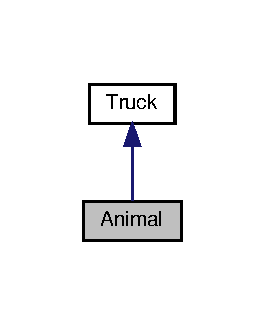
\includegraphics[width=127pt]{class_animal__inherit__graph}
\end{center}
\end{figure}


Collaboration diagram for Animal\+:\nopagebreak
\begin{figure}[H]
\begin{center}
\leavevmode
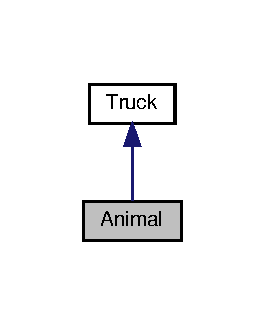
\includegraphics[width=127pt]{class_animal__coll__graph}
\end{center}
\end{figure}
\subsection*{Public Member Functions}
\begin{DoxyCompactItemize}
\item 
\mbox{\Hypertarget{class_animal_afdae9b8c4716472196e8cd62c762f88a}\label{class_animal_afdae9b8c4716472196e8cd62c762f88a}} 
{\bfseries Animal} (string license, bool available, bool \hyperlink{class_truck_a80b8405cf7a15b236fef70116f99c4fb}{registered}, unsigned short \hyperlink{class_truck_a14541fad6d47c606ce4e1bd150a68a23}{capacity}, unsigned short \hyperlink{class_truck_a968fc6b1a6171a03e4254d6615da4ecd}{cargo})
\item 
\mbox{\Hypertarget{class_animal_a1e99083943239209f4fbe79380ea5991}\label{class_animal_a1e99083943239209f4fbe79380ea5991}} 
void {\bfseries info} ()
\end{DoxyCompactItemize}
\subsection*{Static Public Attributes}
\begin{DoxyCompactItemize}
\item 
\mbox{\Hypertarget{class_animal_aa421a3d5192279ca552a62ab3e0517c2}\label{class_animal_aa421a3d5192279ca552a62ab3e0517c2}} 
static float {\bfseries price\+Per\+KG}
\item 
\mbox{\Hypertarget{class_animal_a49d5aaceba02edb1e887131cc596f8ac}\label{class_animal_a49d5aaceba02edb1e887131cc596f8ac}} 
static unordered\+\_\+map$<$ unsigned short, unsigned short $>$ {\bfseries Cap\+Dist}
\end{DoxyCompactItemize}
\subsection*{Additional Inherited Members}


The documentation for this class was generated from the following files\+:\begin{DoxyCompactItemize}
\item 
truck.\+h\item 
truck.\+cpp\end{DoxyCompactItemize}

\hypertarget{class_cant_open_client_file}{}\section{Cant\+Open\+Client\+File Class Reference}
\label{class_cant_open_client_file}\index{Cant\+Open\+Client\+File@{Cant\+Open\+Client\+File}}


Inheritance diagram for Cant\+Open\+Client\+File\+:\nopagebreak
\begin{figure}[H]
\begin{center}
\leavevmode
\includegraphics[width=182pt]{class_cant_open_client_file__inherit__graph}
\end{center}
\end{figure}


Collaboration diagram for Cant\+Open\+Client\+File\+:\nopagebreak
\begin{figure}[H]
\begin{center}
\leavevmode
\includegraphics[width=203pt]{class_cant_open_client_file__coll__graph}
\end{center}
\end{figure}
\subsection*{Public Member Functions}
\begin{DoxyCompactItemize}
\item 
\hyperlink{class_cant_open_client_file_a2185647136543071c3c98199486caf36}{$\sim$\+Cant\+Open\+Client\+File} ()
\item 
\hyperlink{class_cant_open_client_file_a6190eccfaac3cb2f65f3cfd000ed5fb6}{Cant\+Open\+Client\+File} (string \hyperlink{class_cant_open_client_file_aa4aa82cf39a9e960a76d32da6d379b05}{erro})
\begin{DoxyCompactList}\small\item\em Constructor with all data necessary. \end{DoxyCompactList}\end{DoxyCompactItemize}
\subsection*{Public Attributes}
\begin{DoxyCompactItemize}
\item 
string \hyperlink{class_cant_open_client_file_aa4aa82cf39a9e960a76d32da6d379b05}{erro}
\end{DoxyCompactItemize}
\subsection*{Additional Inherited Members}


\subsection{Constructor \& Destructor Documentation}
\mbox{\Hypertarget{class_cant_open_client_file_a2185647136543071c3c98199486caf36}\label{class_cant_open_client_file_a2185647136543071c3c98199486caf36}} 
\index{Cant\+Open\+Client\+File@{Cant\+Open\+Client\+File}!````~Cant\+Open\+Client\+File@{$\sim$\+Cant\+Open\+Client\+File}}
\index{````~Cant\+Open\+Client\+File@{$\sim$\+Cant\+Open\+Client\+File}!Cant\+Open\+Client\+File@{Cant\+Open\+Client\+File}}
\subsubsection{\texorpdfstring{$\sim$\+Cant\+Open\+Client\+File()}{~CantOpenClientFile()}}
{\footnotesize\ttfamily Cant\+Open\+Client\+File\+::$\sim$\+Cant\+Open\+Client\+File (\begin{DoxyParamCaption}{ }\end{DoxyParamCaption})}

Default destructor \mbox{\Hypertarget{class_cant_open_client_file_a6190eccfaac3cb2f65f3cfd000ed5fb6}\label{class_cant_open_client_file_a6190eccfaac3cb2f65f3cfd000ed5fb6}} 
\index{Cant\+Open\+Client\+File@{Cant\+Open\+Client\+File}!Cant\+Open\+Client\+File@{Cant\+Open\+Client\+File}}
\index{Cant\+Open\+Client\+File@{Cant\+Open\+Client\+File}!Cant\+Open\+Client\+File@{Cant\+Open\+Client\+File}}
\subsubsection{\texorpdfstring{Cant\+Open\+Client\+File()}{CantOpenClientFile()}}
{\footnotesize\ttfamily Cant\+Open\+Client\+File\+::\+Cant\+Open\+Client\+File (\begin{DoxyParamCaption}\item[{string}]{erro }\end{DoxyParamCaption})\hspace{0.3cm}{\ttfamily [inline]}}



Constructor with all data necessary. 

This exception is thrown if the program is unable to open the associated file containing the clients


\begin{DoxyParams}{Parameters}
{\em erro} & -\/ Message describing error \\
\hline
\end{DoxyParams}


\subsection{Member Data Documentation}
\mbox{\Hypertarget{class_cant_open_client_file_aa4aa82cf39a9e960a76d32da6d379b05}\label{class_cant_open_client_file_aa4aa82cf39a9e960a76d32da6d379b05}} 
\index{Cant\+Open\+Client\+File@{Cant\+Open\+Client\+File}!erro@{erro}}
\index{erro@{erro}!Cant\+Open\+Client\+File@{Cant\+Open\+Client\+File}}
\subsubsection{\texorpdfstring{erro}{erro}}
{\footnotesize\ttfamily string Cant\+Open\+Client\+File\+::erro}

Message describing error 

The documentation for this class was generated from the following files\+:\begin{DoxyCompactItemize}
\item 
client.\+h\item 
client.\+cpp\end{DoxyCompactItemize}

\hypertarget{class_client}{}\section{Client Class Reference}
\label{class_client}\index{Client@{Client}}


Inheritance diagram for Client\+:\nopagebreak
\begin{figure}[H]
\begin{center}
\leavevmode
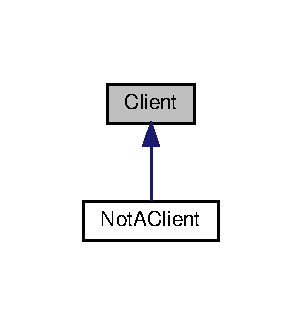
\includegraphics[width=350pt]{class_client__inherit__graph}
\end{center}
\end{figure}
\subsection*{Public Member Functions}
\begin{DoxyCompactItemize}
\item 
\hyperlink{class_client_ab3079953a67493b5da6ffb32d4f14ac7}{Client} (\hyperlink{class_client}{Client} const \&x)
\item 
\hyperlink{class_client_ae51af7aa6b8f591496a8f6a4a87a14bf}{Client} ()
\item 
\hyperlink{class_client_acb0d694a9c7e32a47bd57ead6013b8a9}{Client} (string name, unsigned int \hyperlink{class_client_a1c94dc96a56cb5032573fb1d528517c2}{nif}, float \hyperlink{class_client_a9d5dc70a6eee2fded8217a7983fe5fd0}{money\+\_\+spent}, vector$<$ \hyperlink{class_service}{Service} $\ast$$>$ $\ast$\hyperlink{class_client_a02b601f12b9905edae7e64ded9bde912}{services}=nullptr)
\begin{DoxyCompactList}\small\item\em Constructor with all data necessary. \end{DoxyCompactList}\item 
virtual \hyperlink{class_client_a840e519ca781888cbd54181572ebe3a7}{$\sim$\+Client} ()
\item 
void \hyperlink{class_client_afe8b004559fd1480fb8747c352f167db}{edit\+Client} ()
\begin{DoxyCompactList}\small\item\em Edits the information of a client. \end{DoxyCompactList}\item 
void \hyperlink{class_client_a7f845c33f4aa7b7081ae72d9a16c2d3f}{remove\+Client} (vector$<$ \hyperlink{class_client}{Client} $\ast$$>$ \&clients\+Vector)
\begin{DoxyCompactList}\small\item\em Removes a client. \end{DoxyCompactList}\item 
string \hyperlink{class_client_a5c473ba52d7678744edec9e51052c947}{get\+Name} () const
\begin{DoxyCompactList}\small\item\em Gets the \hyperlink{class_client}{Client}\textquotesingle{}s name. \end{DoxyCompactList}\item 
float \hyperlink{class_client_a226ff919591e7fdfa6c386e9aa5300a5}{get\+Money\+Spent} () const
\begin{DoxyCompactList}\small\item\em Gets the money spent in services. \end{DoxyCompactList}\item 
unsigned \hyperlink{class_client_a35c9fed8cdb36d28fd5e51bd2aee852e}{get\+Nif} () const
\begin{DoxyCompactList}\small\item\em Gets the \hyperlink{class_client}{Client}\textquotesingle{}s identification number. \end{DoxyCompactList}\item 
vector$<$ \hyperlink{class_service}{Service} $\ast$ $>$ $\ast$ \hyperlink{class_client_a13ab3e2d37fde2de5b6a40d4523bb999}{get\+Services\+Vector} ()
\begin{DoxyCompactList}\small\item\em Gets the \hyperlink{class_client}{Client}\textquotesingle{}s bought services. \end{DoxyCompactList}\item 
void \hyperlink{class_client_a1c7f938360e23b3e0e52d17965f88725}{set\+Name} (string name)
\begin{DoxyCompactList}\small\item\em Sets a \hyperlink{class_client}{Client}\textquotesingle{}s name. \end{DoxyCompactList}\item 
void \hyperlink{class_client_a8d0ab1a3c654d361dacde7e1d2b92c94}{set\+Nif} (unsigned \hyperlink{class_client_a1c94dc96a56cb5032573fb1d528517c2}{nif})
\begin{DoxyCompactList}\small\item\em Sets a \hyperlink{class_client}{Client}\textquotesingle{}s identification number. \end{DoxyCompactList}\item 
void \hyperlink{class_client_a65027bc2da365dfdbbf0393ee2697586}{calc\+Money\+Spent} ()
\begin{DoxyCompactList}\small\item\em Calculates the \hyperlink{class_client}{Client}\textquotesingle{}s money spent. \end{DoxyCompactList}\item 
void \hyperlink{class_client_abf36aa7168464608e917fa40f1ba52db}{add\+Service} (\hyperlink{class_service}{Service} $\ast$service)
\begin{DoxyCompactList}\small\item\em Adds a \hyperlink{class_service}{Service} bought by a \hyperlink{class_client}{Client}. \end{DoxyCompactList}\item 
void \hyperlink{class_client_a018c06770de617bb404151e499206355}{remove\+Service} (\hyperlink{class_service}{Service} $\ast$service)
\begin{DoxyCompactList}\small\item\em Removes a service. \end{DoxyCompactList}\item 
bool \hyperlink{class_client_a1cbbbf2ea0d65791314b7640c053197b}{operator$<$} (const \hyperlink{class_client}{Client} \&a) const
\begin{DoxyCompactList}\small\item\em Operator $<$ overloading. \end{DoxyCompactList}\item 
bool \hyperlink{class_client_a5cc669077f776648216ae03461b8c178}{operator==} (const \hyperlink{class_client}{Client} \&client1) const
\begin{DoxyCompactList}\small\item\em Operator == overloading. \end{DoxyCompactList}\end{DoxyCompactItemize}
\subsection*{Static Public Member Functions}
\begin{DoxyCompactItemize}
\item 
static void \hyperlink{class_client_ac18a40ed6975665b7f7661c8dcf7bf1b}{load\+Clients} (vector$<$ \hyperlink{class_client}{Client} $\ast$$>$ \&clients\+Vector)
\begin{DoxyCompactList}\small\item\em Loads the clients. \end{DoxyCompactList}\item 
static void \hyperlink{class_client_aceebaabb74ad1e3e5b30c168e5ef681b}{save\+To\+File} (vector$<$ \hyperlink{class_client}{Client} $\ast$$>$ \&clients\+Vector)
\begin{DoxyCompactList}\small\item\em Saves the clients. \end{DoxyCompactList}\item 
static void \hyperlink{class_client_acd07078857cade36eee66b733de7bc38}{add\+Client} (vector$<$ \hyperlink{class_client}{Client} $\ast$$>$ $\ast$clients\+Vector)
\begin{DoxyCompactList}\small\item\em Adds a \hyperlink{class_client}{Client}. \end{DoxyCompactList}\end{DoxyCompactItemize}
\subsection*{Protected Attributes}
\begin{DoxyCompactItemize}
\item 
float \hyperlink{class_client_a9d5dc70a6eee2fded8217a7983fe5fd0}{money\+\_\+spent} =0
\item 
\mbox{\Hypertarget{class_client_a456e36f9972a8bf3ecdb5f0e70b3bd5d}\label{class_client_a456e36f9972a8bf3ecdb5f0e70b3bd5d}} 
string {\bfseries name}
\item 
unsigned int \hyperlink{class_client_a1c94dc96a56cb5032573fb1d528517c2}{nif}
\item 
vector$<$ \hyperlink{class_service}{Service} $\ast$ $>$ \hyperlink{class_client_a02b601f12b9905edae7e64ded9bde912}{services}
\end{DoxyCompactItemize}
\subsection*{Friends}
\begin{DoxyCompactItemize}
\item 
ostream \& \hyperlink{class_client_a001b1071dc56da194d697f845bbc4b1b}{operator$<$$<$} (ostream \&out, const \hyperlink{class_client}{Client} \&client)
\begin{DoxyCompactList}\small\item\em Operator $<$$<$ overloading. \end{DoxyCompactList}\end{DoxyCompactItemize}


\subsection{Constructor \& Destructor Documentation}
\mbox{\Hypertarget{class_client_ab3079953a67493b5da6ffb32d4f14ac7}\label{class_client_ab3079953a67493b5da6ffb32d4f14ac7}} 
\index{Client@{Client}!Client@{Client}}
\index{Client@{Client}!Client@{Client}}
\subsubsection{\texorpdfstring{Client()}{Client()}\hspace{0.1cm}{\footnotesize\ttfamily [1/3]}}
{\footnotesize\ttfamily Client\+::\+Client (\begin{DoxyParamCaption}\item[{\hyperlink{class_client}{Client} const \&}]{x }\end{DoxyParamCaption})}

Constructor with a \hyperlink{class_client}{Client} Object as parameter 
\begin{DoxyParams}{Parameters}
{\em x} & \hyperlink{class_client}{Client} data that is used to initialize the \hyperlink{class_client}{Client} Object \\
\hline
\end{DoxyParams}
\mbox{\Hypertarget{class_client_ae51af7aa6b8f591496a8f6a4a87a14bf}\label{class_client_ae51af7aa6b8f591496a8f6a4a87a14bf}} 
\index{Client@{Client}!Client@{Client}}
\index{Client@{Client}!Client@{Client}}
\subsubsection{\texorpdfstring{Client()}{Client()}\hspace{0.1cm}{\footnotesize\ttfamily [2/3]}}
{\footnotesize\ttfamily Client\+::\+Client (\begin{DoxyParamCaption}{ }\end{DoxyParamCaption})}

Default Constructor \mbox{\Hypertarget{class_client_acb0d694a9c7e32a47bd57ead6013b8a9}\label{class_client_acb0d694a9c7e32a47bd57ead6013b8a9}} 
\index{Client@{Client}!Client@{Client}}
\index{Client@{Client}!Client@{Client}}
\subsubsection{\texorpdfstring{Client()}{Client()}\hspace{0.1cm}{\footnotesize\ttfamily [3/3]}}
{\footnotesize\ttfamily Client\+::\+Client (\begin{DoxyParamCaption}\item[{string}]{name,  }\item[{unsigned int}]{nif,  }\item[{float}]{money\+\_\+spent,  }\item[{vector$<$ \hyperlink{class_service}{Service} $\ast$$>$ $\ast$}]{services = {\ttfamily nullptr} }\end{DoxyParamCaption})}



Constructor with all data necessary. 

Receives all the data it needs to construct a client properly It is the most used constructor of the three


\begin{DoxyParams}{Parameters}
{\em name} & -\/ Name of the client \\
\hline
{\em nif} & -\/ Identification number of the client \\
\hline
{\em money\+\_\+spent} & -\/ Total amount spent by the client in services \\
\hline
{\em services} & -\/ Pointer to the vector of pointers to Services that the client has bought (none by default) \\
\hline
\end{DoxyParams}
\mbox{\Hypertarget{class_client_a840e519ca781888cbd54181572ebe3a7}\label{class_client_a840e519ca781888cbd54181572ebe3a7}} 
\index{Client@{Client}!````~Client@{$\sim$\+Client}}
\index{````~Client@{$\sim$\+Client}!Client@{Client}}
\subsubsection{\texorpdfstring{$\sim$\+Client()}{~Client()}}
{\footnotesize\ttfamily Client\+::$\sim$\+Client (\begin{DoxyParamCaption}{ }\end{DoxyParamCaption})\hspace{0.3cm}{\ttfamily [virtual]}}

Default Destructor 

\subsection{Member Function Documentation}
\mbox{\Hypertarget{class_client_acd07078857cade36eee66b733de7bc38}\label{class_client_acd07078857cade36eee66b733de7bc38}} 
\index{Client@{Client}!add\+Client@{add\+Client}}
\index{add\+Client@{add\+Client}!Client@{Client}}
\subsubsection{\texorpdfstring{add\+Client()}{addClient()}}
{\footnotesize\ttfamily void Client\+::add\+Client (\begin{DoxyParamCaption}\item[{vector$<$ \hyperlink{class_client}{Client} $\ast$$>$ $\ast$}]{clients\+Vector }\end{DoxyParamCaption})\hspace{0.3cm}{\ttfamily [static]}}



Adds a \hyperlink{class_client}{Client}. 

Adds a \hyperlink{class_client}{Client} to the vector of Clients


\begin{DoxyParams}{Parameters}
{\em clients\+Vector} & -\/ Pointer to the vector of pointers to Clients \\
\hline
\end{DoxyParams}
\begin{DoxyReturn}{Returns}
Returns nothing 
\end{DoxyReturn}
\mbox{\Hypertarget{class_client_abf36aa7168464608e917fa40f1ba52db}\label{class_client_abf36aa7168464608e917fa40f1ba52db}} 
\index{Client@{Client}!add\+Service@{add\+Service}}
\index{add\+Service@{add\+Service}!Client@{Client}}
\subsubsection{\texorpdfstring{add\+Service()}{addService()}}
{\footnotesize\ttfamily void Client\+::add\+Service (\begin{DoxyParamCaption}\item[{\hyperlink{class_service}{Service} $\ast$}]{service }\end{DoxyParamCaption})}



Adds a \hyperlink{class_service}{Service} bought by a \hyperlink{class_client}{Client}. 

Adds a \hyperlink{class_service}{Service} bought by a \hyperlink{class_client}{Client} to the vector of Services


\begin{DoxyParams}{Parameters}
{\em service} & -\/ Pointer to the \hyperlink{class_service}{Service} to he added to the vector of Services \\
\hline
\end{DoxyParams}
\begin{DoxyReturn}{Returns}
Returns nothing 
\end{DoxyReturn}
\mbox{\Hypertarget{class_client_a65027bc2da365dfdbbf0393ee2697586}\label{class_client_a65027bc2da365dfdbbf0393ee2697586}} 
\index{Client@{Client}!calc\+Money\+Spent@{calc\+Money\+Spent}}
\index{calc\+Money\+Spent@{calc\+Money\+Spent}!Client@{Client}}
\subsubsection{\texorpdfstring{calc\+Money\+Spent()}{calcMoneySpent()}}
{\footnotesize\ttfamily void Client\+::calc\+Money\+Spent (\begin{DoxyParamCaption}{ }\end{DoxyParamCaption})}



Calculates the \hyperlink{class_client}{Client}\textquotesingle{}s money spent. 

Computes the money spent by a \hyperlink{class_client}{Client} in services and updates it

\begin{DoxyReturn}{Returns}
Returns nothing 
\end{DoxyReturn}
\mbox{\Hypertarget{class_client_afe8b004559fd1480fb8747c352f167db}\label{class_client_afe8b004559fd1480fb8747c352f167db}} 
\index{Client@{Client}!edit\+Client@{edit\+Client}}
\index{edit\+Client@{edit\+Client}!Client@{Client}}
\subsubsection{\texorpdfstring{edit\+Client()}{editClient()}}
{\footnotesize\ttfamily void Client\+::edit\+Client (\begin{DoxyParamCaption}{ }\end{DoxyParamCaption})}



Edits the information of a client. 

Edits the information of a client by asking

\begin{DoxyReturn}{Returns}
Returns nothing 
\end{DoxyReturn}
\mbox{\Hypertarget{class_client_a226ff919591e7fdfa6c386e9aa5300a5}\label{class_client_a226ff919591e7fdfa6c386e9aa5300a5}} 
\index{Client@{Client}!get\+Money\+Spent@{get\+Money\+Spent}}
\index{get\+Money\+Spent@{get\+Money\+Spent}!Client@{Client}}
\subsubsection{\texorpdfstring{get\+Money\+Spent()}{getMoneySpent()}}
{\footnotesize\ttfamily float Client\+::get\+Money\+Spent (\begin{DoxyParamCaption}{ }\end{DoxyParamCaption}) const}



Gets the money spent in services. 

\begin{DoxyReturn}{Returns}
Returns a float representing the money spent in services by the client 
\end{DoxyReturn}
\mbox{\Hypertarget{class_client_a5c473ba52d7678744edec9e51052c947}\label{class_client_a5c473ba52d7678744edec9e51052c947}} 
\index{Client@{Client}!get\+Name@{get\+Name}}
\index{get\+Name@{get\+Name}!Client@{Client}}
\subsubsection{\texorpdfstring{get\+Name()}{getName()}}
{\footnotesize\ttfamily string Client\+::get\+Name (\begin{DoxyParamCaption}{ }\end{DoxyParamCaption}) const}



Gets the \hyperlink{class_client}{Client}\textquotesingle{}s name. 

\begin{DoxyReturn}{Returns}
Returns a string containing the \hyperlink{class_client}{Client}\textquotesingle{}s name 
\end{DoxyReturn}
\mbox{\Hypertarget{class_client_a35c9fed8cdb36d28fd5e51bd2aee852e}\label{class_client_a35c9fed8cdb36d28fd5e51bd2aee852e}} 
\index{Client@{Client}!get\+Nif@{get\+Nif}}
\index{get\+Nif@{get\+Nif}!Client@{Client}}
\subsubsection{\texorpdfstring{get\+Nif()}{getNif()}}
{\footnotesize\ttfamily unsigned Client\+::get\+Nif (\begin{DoxyParamCaption}{ }\end{DoxyParamCaption}) const}



Gets the \hyperlink{class_client}{Client}\textquotesingle{}s identification number. 

\begin{DoxyReturn}{Returns}
Returns an unsigned 9-\/digit integer containing the \hyperlink{class_client}{Client}\textquotesingle{}s identification number 
\end{DoxyReturn}
\mbox{\Hypertarget{class_client_a13ab3e2d37fde2de5b6a40d4523bb999}\label{class_client_a13ab3e2d37fde2de5b6a40d4523bb999}} 
\index{Client@{Client}!get\+Services\+Vector@{get\+Services\+Vector}}
\index{get\+Services\+Vector@{get\+Services\+Vector}!Client@{Client}}
\subsubsection{\texorpdfstring{get\+Services\+Vector()}{getServicesVector()}}
{\footnotesize\ttfamily vector$<$ \hyperlink{class_service}{Service} $\ast$ $>$ $\ast$ Client\+::get\+Services\+Vector (\begin{DoxyParamCaption}{ }\end{DoxyParamCaption})}



Gets the \hyperlink{class_client}{Client}\textquotesingle{}s bought services. 

\begin{DoxyReturn}{Returns}
Returns an a vector containing pointers to the \hyperlink{class_client}{Client}\textquotesingle{}s bought services 
\end{DoxyReturn}
\mbox{\Hypertarget{class_client_ac18a40ed6975665b7f7661c8dcf7bf1b}\label{class_client_ac18a40ed6975665b7f7661c8dcf7bf1b}} 
\index{Client@{Client}!load\+Clients@{load\+Clients}}
\index{load\+Clients@{load\+Clients}!Client@{Client}}
\subsubsection{\texorpdfstring{load\+Clients()}{loadClients()}}
{\footnotesize\ttfamily void Client\+::load\+Clients (\begin{DoxyParamCaption}\item[{vector$<$ \hyperlink{class_client}{Client} $\ast$$>$ \&}]{clients\+Vector }\end{DoxyParamCaption})\hspace{0.3cm}{\ttfamily [static]}}



Loads the clients. 

Loads the clients into the program by pushing them to a vector


\begin{DoxyParams}{Parameters}
{\em clients\+Vector} & -\/ Vector where the pointers to the Clients are stored \\
\hline
\end{DoxyParams}
\begin{DoxyReturn}{Returns}
Returns nothing 
\end{DoxyReturn}
\mbox{\Hypertarget{class_client_a1cbbbf2ea0d65791314b7640c053197b}\label{class_client_a1cbbbf2ea0d65791314b7640c053197b}} 
\index{Client@{Client}!operator$<$@{operator$<$}}
\index{operator$<$@{operator$<$}!Client@{Client}}
\subsubsection{\texorpdfstring{operator$<$()}{operator<()}}
{\footnotesize\ttfamily bool Client\+::operator$<$ (\begin{DoxyParamCaption}\item[{const \hyperlink{class_client}{Client} \&}]{a }\end{DoxyParamCaption}) const}



Operator $<$ overloading. 

Overload of $<$ operator for comparisons. A \hyperlink{class_client}{Client} is $<$ if his identification number is smaller (as a normal, decimal interpretation)


\begin{DoxyParams}{Parameters}
{\em a} & -\/ \hyperlink{class_client}{Client} Object containing the nif to be compared \\
\hline
\end{DoxyParams}
\begin{DoxyReturn}{Returns}
Returns true if the \hyperlink{class_client}{Client} has a smaller nif 
\end{DoxyReturn}
\mbox{\Hypertarget{class_client_a5cc669077f776648216ae03461b8c178}\label{class_client_a5cc669077f776648216ae03461b8c178}} 
\index{Client@{Client}!operator==@{operator==}}
\index{operator==@{operator==}!Client@{Client}}
\subsubsection{\texorpdfstring{operator==()}{operator==()}}
{\footnotesize\ttfamily bool Client\+::operator== (\begin{DoxyParamCaption}\item[{const \hyperlink{class_client}{Client} \&}]{client1 }\end{DoxyParamCaption}) const}



Operator == overloading. 

Overload of == operator for comparisons. A \hyperlink{class_client}{Client} is == if his identification number is the same


\begin{DoxyParams}{Parameters}
{\em client1} & -\/ \hyperlink{class_client}{Client} Object containing the nif to be compared \\
\hline
\end{DoxyParams}
\begin{DoxyReturn}{Returns}
Returns true if the \hyperlink{class_client}{Client} has an equal nif 
\end{DoxyReturn}
\mbox{\Hypertarget{class_client_a7f845c33f4aa7b7081ae72d9a16c2d3f}\label{class_client_a7f845c33f4aa7b7081ae72d9a16c2d3f}} 
\index{Client@{Client}!remove\+Client@{remove\+Client}}
\index{remove\+Client@{remove\+Client}!Client@{Client}}
\subsubsection{\texorpdfstring{remove\+Client()}{removeClient()}}
{\footnotesize\ttfamily void Client\+::remove\+Client (\begin{DoxyParamCaption}\item[{vector$<$ \hyperlink{class_client}{Client} $\ast$$>$ \&}]{clients\+Vector }\end{DoxyParamCaption})}



Removes a client. 

Removes a client from the vector of Clients if the client has no services bought Throws an exception if the specified client is not found in the vector


\begin{DoxyParams}{Parameters}
{\em clients\+Vector} & -\/ Vector where the pointers to the Clients are stored \\
\hline
\end{DoxyParams}
\begin{DoxyReturn}{Returns}
Returns nothing 
\end{DoxyReturn}
\mbox{\Hypertarget{class_client_a018c06770de617bb404151e499206355}\label{class_client_a018c06770de617bb404151e499206355}} 
\index{Client@{Client}!remove\+Service@{remove\+Service}}
\index{remove\+Service@{remove\+Service}!Client@{Client}}
\subsubsection{\texorpdfstring{remove\+Service()}{removeService()}}
{\footnotesize\ttfamily void Client\+::remove\+Service (\begin{DoxyParamCaption}\item[{\hyperlink{class_service}{Service} $\ast$}]{service }\end{DoxyParamCaption})}



Removes a service. 

Removes a bought service from a \hyperlink{class_client}{Client}


\begin{DoxyParams}{Parameters}
{\em service} & -\/ Pointer to the service to be removed \\
\hline
\end{DoxyParams}
\begin{DoxyReturn}{Returns}
Returns nothing 
\end{DoxyReturn}
\mbox{\Hypertarget{class_client_aceebaabb74ad1e3e5b30c168e5ef681b}\label{class_client_aceebaabb74ad1e3e5b30c168e5ef681b}} 
\index{Client@{Client}!save\+To\+File@{save\+To\+File}}
\index{save\+To\+File@{save\+To\+File}!Client@{Client}}
\subsubsection{\texorpdfstring{save\+To\+File()}{saveToFile()}}
{\footnotesize\ttfamily void Client\+::save\+To\+File (\begin{DoxyParamCaption}\item[{vector$<$ \hyperlink{class_client}{Client} $\ast$$>$ \&}]{clients\+Vector }\end{DoxyParamCaption})\hspace{0.3cm}{\ttfamily [static]}}



Saves the clients. 

Saves the clients the user has added by writing to the clients.\+txt file in the specified format


\begin{DoxyParams}{Parameters}
{\em clients\+Vector} & -\/ Vector where the pointers to the Clients are stored \\
\hline
\end{DoxyParams}
\begin{DoxyReturn}{Returns}
Returns nothing 
\end{DoxyReturn}
\mbox{\Hypertarget{class_client_a1c7f938360e23b3e0e52d17965f88725}\label{class_client_a1c7f938360e23b3e0e52d17965f88725}} 
\index{Client@{Client}!set\+Name@{set\+Name}}
\index{set\+Name@{set\+Name}!Client@{Client}}
\subsubsection{\texorpdfstring{set\+Name()}{setName()}}
{\footnotesize\ttfamily void Client\+::set\+Name (\begin{DoxyParamCaption}\item[{string}]{name }\end{DoxyParamCaption})}



Sets a \hyperlink{class_client}{Client}\textquotesingle{}s name. 

Updates the \hyperlink{class_client}{Client}\textquotesingle{}s name


\begin{DoxyParams}{Parameters}
{\em name} & -\/ String containing the \hyperlink{class_client}{Client}\textquotesingle{}s name to be updated \\
\hline
\end{DoxyParams}
\begin{DoxyReturn}{Returns}
Returns nothing 
\end{DoxyReturn}
\mbox{\Hypertarget{class_client_a8d0ab1a3c654d361dacde7e1d2b92c94}\label{class_client_a8d0ab1a3c654d361dacde7e1d2b92c94}} 
\index{Client@{Client}!set\+Nif@{set\+Nif}}
\index{set\+Nif@{set\+Nif}!Client@{Client}}
\subsubsection{\texorpdfstring{set\+Nif()}{setNif()}}
{\footnotesize\ttfamily void Client\+::set\+Nif (\begin{DoxyParamCaption}\item[{unsigned}]{nif }\end{DoxyParamCaption})}



Sets a \hyperlink{class_client}{Client}\textquotesingle{}s identification number. 

Updates the \hyperlink{class_client}{Client}\textquotesingle{}s identification number


\begin{DoxyParams}{Parameters}
{\em nif} & -\/ an unsigned integer containing the \hyperlink{class_client}{Client}\textquotesingle{}s identification number to be updated \\
\hline
\end{DoxyParams}
\begin{DoxyReturn}{Returns}
Returns nothing 
\end{DoxyReturn}


\subsection{Friends And Related Function Documentation}
\mbox{\Hypertarget{class_client_a001b1071dc56da194d697f845bbc4b1b}\label{class_client_a001b1071dc56da194d697f845bbc4b1b}} 
\index{Client@{Client}!operator$<$$<$@{operator$<$$<$}}
\index{operator$<$$<$@{operator$<$$<$}!Client@{Client}}
\subsubsection{\texorpdfstring{operator$<$$<$}{operator<<}}
{\footnotesize\ttfamily ostream\& operator$<$$<$ (\begin{DoxyParamCaption}\item[{ostream \&}]{out,  }\item[{const \hyperlink{class_client}{Client} \&}]{client }\end{DoxyParamCaption})\hspace{0.3cm}{\ttfamily [friend]}}



Operator $<$$<$ overloading. 

Overload of $<$$<$ operator to allow a \hyperlink{class_client}{Client}\textquotesingle{}s information to be printed


\begin{DoxyParams}{Parameters}
{\em out} & -\/ ostream to allow the chain of ostreams \\
\hline
{\em client} & -\/ \hyperlink{class_client}{Client} Object containing the data to be printed \\
\hline
\end{DoxyParams}
\begin{DoxyReturn}{Returns}
Returns the ostream containing the information to be printed 
\end{DoxyReturn}


\subsection{Member Data Documentation}
\mbox{\Hypertarget{class_client_a9d5dc70a6eee2fded8217a7983fe5fd0}\label{class_client_a9d5dc70a6eee2fded8217a7983fe5fd0}} 
\index{Client@{Client}!money\+\_\+spent@{money\+\_\+spent}}
\index{money\+\_\+spent@{money\+\_\+spent}!Client@{Client}}
\subsubsection{\texorpdfstring{money\+\_\+spent}{money\_spent}}
{\footnotesize\ttfamily float Client\+::money\+\_\+spent =0\hspace{0.3cm}{\ttfamily [protected]}}

Total money spent in services \mbox{\Hypertarget{class_client_a1c94dc96a56cb5032573fb1d528517c2}\label{class_client_a1c94dc96a56cb5032573fb1d528517c2}} 
\index{Client@{Client}!nif@{nif}}
\index{nif@{nif}!Client@{Client}}
\subsubsection{\texorpdfstring{nif}{nif}}
{\footnotesize\ttfamily unsigned int Client\+::nif\hspace{0.3cm}{\ttfamily [protected]}}

\hyperlink{class_client}{Client}\textquotesingle{}s Identification -\/ used whenever comparing and verifying clients \mbox{\Hypertarget{class_client_a02b601f12b9905edae7e64ded9bde912}\label{class_client_a02b601f12b9905edae7e64ded9bde912}} 
\index{Client@{Client}!services@{services}}
\index{services@{services}!Client@{Client}}
\subsubsection{\texorpdfstring{services}{services}}
{\footnotesize\ttfamily vector$<$\hyperlink{class_service}{Service}$\ast$$>$ Client\+::services\hspace{0.3cm}{\ttfamily [protected]}}

\hyperlink{class_client}{Client}\textquotesingle{}s vector of bought Services 

The documentation for this class was generated from the following files\+:\begin{DoxyCompactItemize}
\item 
client.\+h\item 
client.\+cpp\end{DoxyCompactItemize}

\hypertarget{class_client_in_vector}{}\section{Client\+In\+Vector Class Reference}
\label{class_client_in_vector}\index{Client\+In\+Vector@{Client\+In\+Vector}}


Inheritance diagram for Client\+In\+Vector\+:
\nopagebreak
\begin{figure}[H]
\begin{center}
\leavevmode
\includegraphics[width=159pt]{class_client_in_vector__inherit__graph}
\end{center}
\end{figure}


Collaboration diagram for Client\+In\+Vector\+:
\nopagebreak
\begin{figure}[H]
\begin{center}
\leavevmode
\includegraphics[width=192pt]{class_client_in_vector__coll__graph}
\end{center}
\end{figure}
\subsection*{Public Member Functions}
\begin{DoxyCompactItemize}
\item 
\hyperlink{class_client_in_vector_aa5187e63a59d3340d1287d7a91b4106a}{$\sim$\+Client\+In\+Vector} ()
\item 
\hyperlink{class_client_in_vector_a10ec0356f39e99be9205d5c0f6897652}{Client\+In\+Vector} (unsigned nif\+\_\+n, string \hyperlink{class_client_in_vector_a65d04995fa02a6f36d00540120be34b5}{erro})
\begin{DoxyCompactList}\small\item\em Constructor with all data necessary. \end{DoxyCompactList}\item 
unsigned int \hyperlink{class_client_in_vector_adab501aba615f5d9b69bbe7a28053801}{get\+Nif} () const
\begin{DoxyCompactList}\small\item\em Gets identification number. \end{DoxyCompactList}\end{DoxyCompactItemize}
\subsection*{Public Attributes}
\begin{DoxyCompactItemize}
\item 
string \hyperlink{class_client_in_vector_a65d04995fa02a6f36d00540120be34b5}{erro}
\item 
\mbox{\Hypertarget{class_client_in_vector_a8a7af8db098724eb214125a67c733955}\label{class_client_in_vector_a8a7af8db098724eb214125a67c733955}} 
unsigned {\bfseries nif}
\end{DoxyCompactItemize}
\subsection*{Additional Inherited Members}


\subsection{Constructor \& Destructor Documentation}
\mbox{\Hypertarget{class_client_in_vector_aa5187e63a59d3340d1287d7a91b4106a}\label{class_client_in_vector_aa5187e63a59d3340d1287d7a91b4106a}} 
\index{Client\+In\+Vector@{Client\+In\+Vector}!````~Client\+In\+Vector@{$\sim$\+Client\+In\+Vector}}
\index{````~Client\+In\+Vector@{$\sim$\+Client\+In\+Vector}!Client\+In\+Vector@{Client\+In\+Vector}}
\subsubsection{\texorpdfstring{$\sim$\+Client\+In\+Vector()}{~ClientInVector()}}
{\footnotesize\ttfamily Client\+In\+Vector\+::$\sim$\+Client\+In\+Vector (\begin{DoxyParamCaption}{ }\end{DoxyParamCaption})}

Default destructor \mbox{\Hypertarget{class_client_in_vector_a10ec0356f39e99be9205d5c0f6897652}\label{class_client_in_vector_a10ec0356f39e99be9205d5c0f6897652}} 
\index{Client\+In\+Vector@{Client\+In\+Vector}!Client\+In\+Vector@{Client\+In\+Vector}}
\index{Client\+In\+Vector@{Client\+In\+Vector}!Client\+In\+Vector@{Client\+In\+Vector}}
\subsubsection{\texorpdfstring{Client\+In\+Vector()}{ClientInVector()}}
{\footnotesize\ttfamily Client\+In\+Vector\+::\+Client\+In\+Vector (\begin{DoxyParamCaption}\item[{unsigned}]{nif\+\_\+n,  }\item[{string}]{erro }\end{DoxyParamCaption})\hspace{0.3cm}{\ttfamily [inline]}}



Constructor with all data necessary. 

This exception is thrown if the \hyperlink{class_client}{Client} being searched for is already in the Clients vector


\begin{DoxyParams}{Parameters}
{\em nif\+\_\+n} & -\/ Identification number of the client \\
\hline
{\em erro} & -\/ Message describing error \\
\hline
\end{DoxyParams}


\subsection{Member Function Documentation}
\mbox{\Hypertarget{class_client_in_vector_adab501aba615f5d9b69bbe7a28053801}\label{class_client_in_vector_adab501aba615f5d9b69bbe7a28053801}} 
\index{Client\+In\+Vector@{Client\+In\+Vector}!get\+Nif@{get\+Nif}}
\index{get\+Nif@{get\+Nif}!Client\+In\+Vector@{Client\+In\+Vector}}
\subsubsection{\texorpdfstring{get\+Nif()}{getNif()}}
{\footnotesize\ttfamily unsigned int Client\+In\+Vector\+::get\+Nif (\begin{DoxyParamCaption}{ }\end{DoxyParamCaption}) const\hspace{0.3cm}{\ttfamily [inline]}}



Gets identification number. 

Returns identification number of the client

\begin{DoxyReturn}{Returns}
Returns an unsigned integer containing the identification number 
\end{DoxyReturn}


\subsection{Member Data Documentation}
\mbox{\Hypertarget{class_client_in_vector_a65d04995fa02a6f36d00540120be34b5}\label{class_client_in_vector_a65d04995fa02a6f36d00540120be34b5}} 
\index{Client\+In\+Vector@{Client\+In\+Vector}!erro@{erro}}
\index{erro@{erro}!Client\+In\+Vector@{Client\+In\+Vector}}
\subsubsection{\texorpdfstring{erro}{erro}}
{\footnotesize\ttfamily string Client\+In\+Vector\+::erro}

Message describing error 

The documentation for this class was generated from the following files\+:\begin{DoxyCompactItemize}
\item 
client.\+h\item 
client.\+cpp\end{DoxyCompactItemize}

\hypertarget{class_company}{}\section{Company Class Reference}
\label{class_company}\index{Company@{Company}}
\subsection*{Public Member Functions}
\begin{DoxyCompactItemize}
\item 
\mbox{\Hypertarget{class_company_ae818941883e08e25e93373f29922f9b3}\label{class_company_ae818941883e08e25e93373f29922f9b3}} 
vector$<$ \hyperlink{class_service}{Service} $\ast$ $>$ $\ast$ {\bfseries get\+Vector\+Services\+Finished} ()
\item 
\mbox{\Hypertarget{class_company_ab83ddbd16558f0e99efa7c56878e0ec8}\label{class_company_ab83ddbd16558f0e99efa7c56878e0ec8}} 
vector$<$ \hyperlink{class_service}{Service} $\ast$ $>$ $\ast$ {\bfseries get\+Vector\+Services\+On\+Transit} ()
\item 
\mbox{\Hypertarget{class_company_adffe3680413d999c922858c88fbd18a6}\label{class_company_adffe3680413d999c922858c88fbd18a6}} 
vector$<$ \hyperlink{class_service}{Service} $\ast$ $>$ $\ast$ {\bfseries get\+Vector\+Services\+On\+Queue} ()
\item 
\mbox{\Hypertarget{class_company_a16693c2e4bf9a932e15926c37c21485f}\label{class_company_a16693c2e4bf9a932e15926c37c21485f}} 
vector$<$ \hyperlink{class_client}{Client} $\ast$ $>$ $\ast$ {\bfseries get\+Vector\+Clients} ()
\item 
\mbox{\Hypertarget{class_company_a78feb735977ce59f253a30082dbf24b6}\label{class_company_a78feb735977ce59f253a30082dbf24b6}} 
vector$<$ \hyperlink{class_truck}{Truck} $\ast$ $>$ $\ast$ {\bfseries get\+Vector\+Trucks} ()
\item 
\mbox{\Hypertarget{class_company_ae8efdaf521467fd204c8d272f4469679}\label{class_company_ae8efdaf521467fd204c8d272f4469679}} 
\hyperlink{class_client}{Client} $\ast$ {\bfseries get\+Client} (unsigned nif)
\item 
\mbox{\Hypertarget{class_company_acb9c7285e4ca619899017bd1221a1d27}\label{class_company_acb9c7285e4ca619899017bd1221a1d27}} 
\hyperlink{class_truck}{Truck} $\ast$ {\bfseries get\+Truck} (string license)
\end{DoxyCompactItemize}
\subsection*{Static Public Member Functions}
\begin{DoxyCompactItemize}
\item 
\mbox{\Hypertarget{class_company_a453411f6ef4bab2e878867302fdcf484}\label{class_company_a453411f6ef4bab2e878867302fdcf484}} 
static \hyperlink{class_company}{Company} $\ast$ {\bfseries get\+Company} ()
\end{DoxyCompactItemize}
\subsection*{Public Attributes}
\begin{DoxyCompactItemize}
\item 
\mbox{\Hypertarget{class_company_a0671d8c8afcbe73e5719eac7db205859}\label{class_company_a0671d8c8afcbe73e5719eac7db205859}} 
bool {\bfseries services\+\_\+finished\+\_\+changed} =false
\item 
\mbox{\Hypertarget{class_company_aeac99d209136e732106bc0a3dad7d5d1}\label{class_company_aeac99d209136e732106bc0a3dad7d5d1}} 
bool {\bfseries services\+\_\+on\+\_\+transit\+\_\+changed} =false
\item 
\mbox{\Hypertarget{class_company_a7f986eaf19517385d257ecf74a1a970a}\label{class_company_a7f986eaf19517385d257ecf74a1a970a}} 
bool {\bfseries services\+\_\+on\+\_\+queue\+\_\+changed} =false
\item 
\mbox{\Hypertarget{class_company_ab565013c5770e9ac94cc7f2875917f45}\label{class_company_ab565013c5770e9ac94cc7f2875917f45}} 
bool {\bfseries clients\+\_\+changed} =false
\item 
\mbox{\Hypertarget{class_company_ae9ee930a4a92e6f048960e486d2783dd}\label{class_company_ae9ee930a4a92e6f048960e486d2783dd}} 
bool {\bfseries trucks\+\_\+changed} =false
\end{DoxyCompactItemize}


The documentation for this class was generated from the following files\+:\begin{DoxyCompactItemize}
\item 
company.\+h\item 
company.\+cpp\item 
Servicos-\/do-\/\+Ze-\/\+Manel.\+cpp\end{DoxyCompactItemize}

\hypertarget{class_congelation}{}\section{Congelation Class Reference}
\label{class_congelation}\index{Congelation@{Congelation}}


Inheritance diagram for Congelation\+:\nopagebreak
\begin{figure}[H]
\begin{center}
\leavevmode
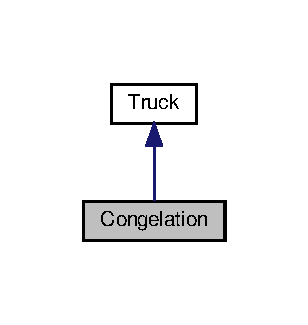
\includegraphics[width=148pt]{class_congelation__inherit__graph}
\end{center}
\end{figure}


Collaboration diagram for Congelation\+:\nopagebreak
\begin{figure}[H]
\begin{center}
\leavevmode
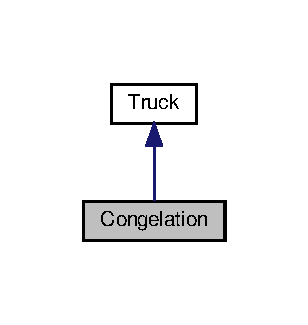
\includegraphics[width=148pt]{class_congelation__coll__graph}
\end{center}
\end{figure}
\subsection*{Public Member Functions}
\begin{DoxyCompactItemize}
\item 
\hyperlink{class_congelation_a320f8a45809dbe0d770f9f77d49b3629}{Congelation} (string license, bool \hyperlink{class_truck_a4189fe5ed32f6084459a9c5ae1eb7c2a}{available}, bool \hyperlink{class_truck_a80b8405cf7a15b236fef70116f99c4fb}{registered}, unsigned short \hyperlink{class_truck_ab004524786ae7aebf7c7bdb5e1599696}{capacity}, unsigned short cargo)
\begin{DoxyCompactList}\small\item\em constructor for this subclass that calls the one from superclass \end{DoxyCompactList}\item 
\hyperlink{class_congelation_a7aa24e7127ec7c1d9d01043b665ae66f}{$\sim$\+Congelation} ()
\begin{DoxyCompactList}\small\item\em Default destructor. \end{DoxyCompactList}\item 
void \hyperlink{class_congelation_ac2f7cb9aeeeb9428a9a973e6a2c63942}{info} ()
\begin{DoxyCompactList}\small\item\em Prints more specific information about this truck\textquotesingle{}s subclass. \end{DoxyCompactList}\item 
type \hyperlink{class_congelation_a5026bd6791faeae03fbf1ad84f9bbc08}{get\+Type} ()
\begin{DoxyCompactList}\small\item\em return type of truck \end{DoxyCompactList}\end{DoxyCompactItemize}
\subsection*{Static Public Attributes}
\begin{DoxyCompactItemize}
\item 
static unordered\+\_\+map$<$ Temperature\+\_\+enum, float $>$ \hyperlink{class_congelation_aa0cf9fa825aa450ff04d58e5e733706b}{temp\+Mul}
\item 
static map$<$ unsigned, unsigned $>$ \hyperlink{class_congelation_aaa0f7881a3e1e58c35176bdd22e27425}{Cap\+Dist}
\item 
\mbox{\Hypertarget{class_congelation_ab30061aebb6a0fa59ec3f40e9de0ca34}\label{class_congelation_ab30061aebb6a0fa59ec3f40e9de0ca34}} 
static float {\bfseries price\+Per\+KG}
\end{DoxyCompactItemize}
\subsection*{Additional Inherited Members}


\subsection{Constructor \& Destructor Documentation}
\mbox{\Hypertarget{class_congelation_a320f8a45809dbe0d770f9f77d49b3629}\label{class_congelation_a320f8a45809dbe0d770f9f77d49b3629}} 
\index{Congelation@{Congelation}!Congelation@{Congelation}}
\index{Congelation@{Congelation}!Congelation@{Congelation}}
\subsubsection{\texorpdfstring{Congelation()}{Congelation()}}
{\footnotesize\ttfamily Congelation\+::\+Congelation (\begin{DoxyParamCaption}\item[{string}]{license,  }\item[{bool}]{available,  }\item[{bool}]{registered,  }\item[{unsigned short}]{capacity,  }\item[{unsigned short}]{cargo }\end{DoxyParamCaption})}



constructor for this subclass that calls the one from superclass 

\begin{DoxyReturn}{Returns}
Returns nothing 
\end{DoxyReturn}
\mbox{\Hypertarget{class_congelation_a7aa24e7127ec7c1d9d01043b665ae66f}\label{class_congelation_a7aa24e7127ec7c1d9d01043b665ae66f}} 
\index{Congelation@{Congelation}!````~Congelation@{$\sim$\+Congelation}}
\index{````~Congelation@{$\sim$\+Congelation}!Congelation@{Congelation}}
\subsubsection{\texorpdfstring{$\sim$\+Congelation()}{~Congelation()}}
{\footnotesize\ttfamily Congelation\+::$\sim$\+Congelation (\begin{DoxyParamCaption}{ }\end{DoxyParamCaption})\hspace{0.3cm}{\ttfamily [inline]}}



Default destructor. 

\begin{DoxyReturn}{Returns}
Returns nothing 
\end{DoxyReturn}


\subsection{Member Function Documentation}
\mbox{\Hypertarget{class_congelation_a5026bd6791faeae03fbf1ad84f9bbc08}\label{class_congelation_a5026bd6791faeae03fbf1ad84f9bbc08}} 
\index{Congelation@{Congelation}!get\+Type@{get\+Type}}
\index{get\+Type@{get\+Type}!Congelation@{Congelation}}
\subsubsection{\texorpdfstring{get\+Type()}{getType()}}
{\footnotesize\ttfamily type Congelation\+::get\+Type (\begin{DoxyParamCaption}{ }\end{DoxyParamCaption})\hspace{0.3cm}{\ttfamily [virtual]}}



return type of truck 

\begin{DoxyReturn}{Returns}
Returns type of truck 
\end{DoxyReturn}


Reimplemented from \hyperlink{class_truck_a24406caf4d09be7f3eff069ce6bc015b}{Truck}.

\mbox{\Hypertarget{class_congelation_ac2f7cb9aeeeb9428a9a973e6a2c63942}\label{class_congelation_ac2f7cb9aeeeb9428a9a973e6a2c63942}} 
\index{Congelation@{Congelation}!info@{info}}
\index{info@{info}!Congelation@{Congelation}}
\subsubsection{\texorpdfstring{info()}{info()}}
{\footnotesize\ttfamily void Congelation\+::info (\begin{DoxyParamCaption}{ }\end{DoxyParamCaption})\hspace{0.3cm}{\ttfamily [virtual]}}



Prints more specific information about this truck\textquotesingle{}s subclass. 

\begin{DoxyReturn}{Returns}
Returns nothing 
\end{DoxyReturn}


Reimplemented from \hyperlink{class_truck_a38f09eab2822524e355ecf6d0a13f7de}{Truck}.



\subsection{Member Data Documentation}
\mbox{\Hypertarget{class_congelation_aaa0f7881a3e1e58c35176bdd22e27425}\label{class_congelation_aaa0f7881a3e1e58c35176bdd22e27425}} 
\index{Congelation@{Congelation}!Cap\+Dist@{Cap\+Dist}}
\index{Cap\+Dist@{Cap\+Dist}!Congelation@{Congelation}}
\subsubsection{\texorpdfstring{Cap\+Dist}{CapDist}}
{\footnotesize\ttfamily map$<$ unsigned, unsigned $>$ Congelation\+::\+Cap\+Dist\hspace{0.3cm}{\ttfamily [static]}}

holds how many trucks of this have x capacity being that the latter is the key \mbox{\Hypertarget{class_congelation_aa0cf9fa825aa450ff04d58e5e733706b}\label{class_congelation_aa0cf9fa825aa450ff04d58e5e733706b}} 
\index{Congelation@{Congelation}!temp\+Mul@{temp\+Mul}}
\index{temp\+Mul@{temp\+Mul}!Congelation@{Congelation}}
\subsubsection{\texorpdfstring{temp\+Mul}{tempMul}}
{\footnotesize\ttfamily unordered\+\_\+map$<$ Temperature\+\_\+enum, float $>$ Congelation\+::temp\+Mul\hspace{0.3cm}{\ttfamily [static]}}

will hold price multipliers depending on the service 

The documentation for this class was generated from the following files\+:\begin{DoxyCompactItemize}
\item 
truck.\+h\item 
truck.\+cpp\end{DoxyCompactItemize}

\hypertarget{class_date}{}\section{Date Class Reference}
\label{class_date}\index{Date@{Date}}
\subsection*{Public Member Functions}
\begin{DoxyCompactItemize}
\item 
\hyperlink{class_date_a4e59ed4ba66eec61c27460c5d09fa1bd}{Date} ()
\item 
\hyperlink{class_date_ade4b469433b7966cc034cbcc6799233b}{$\sim$\+Date} ()
\item 
\hyperlink{class_date_a5277264fbbce7f4ebfcbcc362d6d62e7}{Date} (unsigned year, unsigned short month, unsigned short day, unsigned short hour, unsigned short minute)
\begin{DoxyCompactList}\small\item\em Constructor with data. \end{DoxyCompactList}\item 
\hyperlink{class_date_a5532efafed41fd5f8e013a61313200dc}{Date} (string date)
\begin{DoxyCompactList}\small\item\em Constructor with string. \end{DoxyCompactList}\item 
unsigned int \hyperlink{class_date_aa1e4066bffc24af79f604dabce27e3cc}{get\+Year} () const
\begin{DoxyCompactList}\small\item\em Gets year. \end{DoxyCompactList}\item 
unsigned short \hyperlink{class_date_ad077bd6ae19462875a8bd10aed9a6233}{get\+Month} () const
\begin{DoxyCompactList}\small\item\em Gets month. \end{DoxyCompactList}\item 
unsigned short \hyperlink{class_date_af02c2f0b61b6e14efbc3ccb0f7f0d567}{get\+Day} () const
\begin{DoxyCompactList}\small\item\em Gets day. \end{DoxyCompactList}\item 
unsigned short \hyperlink{class_date_a49673a3830aada7b4b55616b5848c843}{get\+Hour} () const
\begin{DoxyCompactList}\small\item\em Gets hour. \end{DoxyCompactList}\item 
void \hyperlink{class_date_a39aed5716d41cecafc37be6a11556112}{set\+Hour} (int hour)
\begin{DoxyCompactList}\small\item\em Gets minutes. \end{DoxyCompactList}\item 
\mbox{\Hypertarget{class_date_aa4d5c4e15ec04ff5fa18755d76acefe0}\label{class_date_aa4d5c4e15ec04ff5fa18755d76acefe0}} 
unsigned short {\bfseries get\+Minute} () const
\item 
string \hyperlink{class_date_ac33192f734973548e97e9b5d8da44a5b}{get\+Date} () const
\begin{DoxyCompactList}\small\item\em Gets date as a string. \end{DoxyCompactList}\item 
string \hyperlink{class_date_a1c481aea42a3a310364f9a97661bee14}{get\+Date\+W\+Hour} () const
\begin{DoxyCompactList}\small\item\em Gets date as a string. \end{DoxyCompactList}\item 
void \hyperlink{class_date_a262bd42a1ed4378fa115dab321096736}{set\+Year} (unsigned year)
\begin{DoxyCompactList}\small\item\em Sets year. \end{DoxyCompactList}\item 
void \hyperlink{class_date_a6f2ab890b1935488aaa604b77caac4ae}{set\+Month} (unsigned short month)
\begin{DoxyCompactList}\small\item\em Sets month. \end{DoxyCompactList}\item 
void \hyperlink{class_date_a61e8103c09406f067992e15f36a7f910}{set\+Day} (unsigned short day)
\begin{DoxyCompactList}\small\item\em Sets day. \end{DoxyCompactList}\item 
void \hyperlink{class_date_a8c5fc0dd7ecf3bae6a1de5146fc566e4}{set\+Date} (unsigned year, unsigned short month, unsigned short day)
\begin{DoxyCompactList}\small\item\em Sets date. \end{DoxyCompactList}\item 
bool \hyperlink{class_date_a7d9aaa9db591413e21c8b85fdae130ad}{is\+Valid} ()
\begin{DoxyCompactList}\small\item\em Verifies \hyperlink{class_date}{Date}. \end{DoxyCompactList}\item 
void \hyperlink{class_date_a37f8fc7ca1692df7a8b265099c061721}{show} () const
\begin{DoxyCompactList}\small\item\em Prints \hyperlink{class_date}{Date}. \end{DoxyCompactList}\end{DoxyCompactItemize}


\subsection{Constructor \& Destructor Documentation}
\mbox{\Hypertarget{class_date_a4e59ed4ba66eec61c27460c5d09fa1bd}\label{class_date_a4e59ed4ba66eec61c27460c5d09fa1bd}} 
\index{Date@{Date}!Date@{Date}}
\index{Date@{Date}!Date@{Date}}
\subsubsection{\texorpdfstring{Date()}{Date()}\hspace{0.1cm}{\footnotesize\ttfamily [1/3]}}
{\footnotesize\ttfamily Date\+::\+Date (\begin{DoxyParamCaption}{ }\end{DoxyParamCaption})}

Default constructor \mbox{\Hypertarget{class_date_ade4b469433b7966cc034cbcc6799233b}\label{class_date_ade4b469433b7966cc034cbcc6799233b}} 
\index{Date@{Date}!````~Date@{$\sim$\+Date}}
\index{````~Date@{$\sim$\+Date}!Date@{Date}}
\subsubsection{\texorpdfstring{$\sim$\+Date()}{~Date()}}
{\footnotesize\ttfamily Date\+::$\sim$\+Date (\begin{DoxyParamCaption}{ }\end{DoxyParamCaption})}

Default destructor \mbox{\Hypertarget{class_date_a5277264fbbce7f4ebfcbcc362d6d62e7}\label{class_date_a5277264fbbce7f4ebfcbcc362d6d62e7}} 
\index{Date@{Date}!Date@{Date}}
\index{Date@{Date}!Date@{Date}}
\subsubsection{\texorpdfstring{Date()}{Date()}\hspace{0.1cm}{\footnotesize\ttfamily [2/3]}}
{\footnotesize\ttfamily Date\+::\+Date (\begin{DoxyParamCaption}\item[{unsigned}]{year,  }\item[{unsigned short}]{month,  }\item[{unsigned short}]{day,  }\item[{unsigned short}]{hour,  }\item[{unsigned short}]{minute }\end{DoxyParamCaption})}



Constructor with data. 

Constructs the object by receiving all the necessary information


\begin{DoxyParams}{Parameters}
{\em year} & -\/ year of the \hyperlink{class_date}{Date} \\
\hline
{\em month} & -\/ mpnth of the \hyperlink{class_date}{Date} \\
\hline
{\em day} & -\/ day of the \hyperlink{class_date}{Date} \\
\hline
{\em hour} & -\/ hour of the \hyperlink{class_date}{Date} \\
\hline
{\em minute} & -\/ minute of the \hyperlink{class_date}{Date} \\
\hline
\end{DoxyParams}
\mbox{\Hypertarget{class_date_a5532efafed41fd5f8e013a61313200dc}\label{class_date_a5532efafed41fd5f8e013a61313200dc}} 
\index{Date@{Date}!Date@{Date}}
\index{Date@{Date}!Date@{Date}}
\subsubsection{\texorpdfstring{Date()}{Date()}\hspace{0.1cm}{\footnotesize\ttfamily [3/3]}}
{\footnotesize\ttfamily Date\+::\+Date (\begin{DoxyParamCaption}\item[{string}]{date }\end{DoxyParamCaption})}



Constructor with string. 

Constructs the object by parsing the received string


\begin{DoxyParams}{Parameters}
{\em date} & -\/ string containing all the informatio in the format \char`\"{}yyyy/mm/dd/hh/mm\char`\"{} \\
\hline
\end{DoxyParams}


\subsection{Member Function Documentation}
\mbox{\Hypertarget{class_date_ac33192f734973548e97e9b5d8da44a5b}\label{class_date_ac33192f734973548e97e9b5d8da44a5b}} 
\index{Date@{Date}!get\+Date@{get\+Date}}
\index{get\+Date@{get\+Date}!Date@{Date}}
\subsubsection{\texorpdfstring{get\+Date()}{getDate()}}
{\footnotesize\ttfamily string Date\+::get\+Date (\begin{DoxyParamCaption}{ }\end{DoxyParamCaption}) const}



Gets date as a string. 

Returns the date as a string in the format \char`\"{}yyyy/mm/dd/hh/mm\char`\"{} for file-\/writing purposes

\begin{DoxyReturn}{Returns}
the date as a string in the format \char`\"{}yyyy/mm/dd/hh/mm\char`\"{} 
\end{DoxyReturn}
\mbox{\Hypertarget{class_date_a1c481aea42a3a310364f9a97661bee14}\label{class_date_a1c481aea42a3a310364f9a97661bee14}} 
\index{Date@{Date}!get\+Date\+W\+Hour@{get\+Date\+W\+Hour}}
\index{get\+Date\+W\+Hour@{get\+Date\+W\+Hour}!Date@{Date}}
\subsubsection{\texorpdfstring{get\+Date\+W\+Hour()}{getDateWHour()}}
{\footnotesize\ttfamily string Date\+::get\+Date\+W\+Hour (\begin{DoxyParamCaption}{ }\end{DoxyParamCaption}) const}



Gets date as a string. 

Returns the date as a string in the format \char`\"{}yyyy/mm/dd/hh/mm\char`\"{} for printing purposes

\begin{DoxyReturn}{Returns}
the date as a string in the format \char`\"{}yyyy/mm/dd/hh/mm\char`\"{} 
\end{DoxyReturn}
\mbox{\Hypertarget{class_date_af02c2f0b61b6e14efbc3ccb0f7f0d567}\label{class_date_af02c2f0b61b6e14efbc3ccb0f7f0d567}} 
\index{Date@{Date}!get\+Day@{get\+Day}}
\index{get\+Day@{get\+Day}!Date@{Date}}
\subsubsection{\texorpdfstring{get\+Day()}{getDay()}}
{\footnotesize\ttfamily unsigned short Date\+::get\+Day (\begin{DoxyParamCaption}{ }\end{DoxyParamCaption}) const}



Gets day. 

Returns the day of the \hyperlink{class_date}{Date}

\begin{DoxyReturn}{Returns}
Returns the day of the \hyperlink{class_date}{Date} 
\end{DoxyReturn}
\mbox{\Hypertarget{class_date_a49673a3830aada7b4b55616b5848c843}\label{class_date_a49673a3830aada7b4b55616b5848c843}} 
\index{Date@{Date}!get\+Hour@{get\+Hour}}
\index{get\+Hour@{get\+Hour}!Date@{Date}}
\subsubsection{\texorpdfstring{get\+Hour()}{getHour()}}
{\footnotesize\ttfamily unsigned short Date\+::get\+Hour (\begin{DoxyParamCaption}{ }\end{DoxyParamCaption}) const}



Gets hour. 

Returns the hour of the \hyperlink{class_date}{Date}

\begin{DoxyReturn}{Returns}
Returns the hour of the \hyperlink{class_date}{Date} 
\end{DoxyReturn}
\mbox{\Hypertarget{class_date_ad077bd6ae19462875a8bd10aed9a6233}\label{class_date_ad077bd6ae19462875a8bd10aed9a6233}} 
\index{Date@{Date}!get\+Month@{get\+Month}}
\index{get\+Month@{get\+Month}!Date@{Date}}
\subsubsection{\texorpdfstring{get\+Month()}{getMonth()}}
{\footnotesize\ttfamily unsigned short Date\+::get\+Month (\begin{DoxyParamCaption}{ }\end{DoxyParamCaption}) const}



Gets month. 

Returns the month of the \hyperlink{class_date}{Date}

\begin{DoxyReturn}{Returns}
Returns the month of the \hyperlink{class_date}{Date} 
\end{DoxyReturn}
\mbox{\Hypertarget{class_date_aa1e4066bffc24af79f604dabce27e3cc}\label{class_date_aa1e4066bffc24af79f604dabce27e3cc}} 
\index{Date@{Date}!get\+Year@{get\+Year}}
\index{get\+Year@{get\+Year}!Date@{Date}}
\subsubsection{\texorpdfstring{get\+Year()}{getYear()}}
{\footnotesize\ttfamily unsigned Date\+::get\+Year (\begin{DoxyParamCaption}{ }\end{DoxyParamCaption}) const}



Gets year. 

Returns the year of the \hyperlink{class_date}{Date}

\begin{DoxyReturn}{Returns}
Returns the year of the \hyperlink{class_date}{Date} 
\end{DoxyReturn}
\mbox{\Hypertarget{class_date_a7d9aaa9db591413e21c8b85fdae130ad}\label{class_date_a7d9aaa9db591413e21c8b85fdae130ad}} 
\index{Date@{Date}!is\+Valid@{is\+Valid}}
\index{is\+Valid@{is\+Valid}!Date@{Date}}
\subsubsection{\texorpdfstring{is\+Valid()}{isValid()}}
{\footnotesize\ttfamily bool Date\+::is\+Valid (\begin{DoxyParamCaption}{ }\end{DoxyParamCaption})}



Verifies \hyperlink{class_date}{Date}. 

Verifies if the \hyperlink{class_date}{Date} is valid

\begin{DoxyReturn}{Returns}
Returns true if the \hyperlink{class_date}{Date} is valid 
\end{DoxyReturn}
\mbox{\Hypertarget{class_date_a8c5fc0dd7ecf3bae6a1de5146fc566e4}\label{class_date_a8c5fc0dd7ecf3bae6a1de5146fc566e4}} 
\index{Date@{Date}!set\+Date@{set\+Date}}
\index{set\+Date@{set\+Date}!Date@{Date}}
\subsubsection{\texorpdfstring{set\+Date()}{setDate()}}
{\footnotesize\ttfamily void Date\+::set\+Date (\begin{DoxyParamCaption}\item[{unsigned}]{year,  }\item[{unsigned short}]{month,  }\item[{unsigned short}]{day }\end{DoxyParamCaption})}



Sets date. 

Sets the date by receiving all the data necessary


\begin{DoxyParams}{Parameters}
{\em year} & -\/ year to be set \\
\hline
{\em month} & -\/ month to be set \\
\hline
{\em day} & -\/ day to be set \\
\hline
\end{DoxyParams}
\begin{DoxyReturn}{Returns}
Returns nothing 
\end{DoxyReturn}
\mbox{\Hypertarget{class_date_a61e8103c09406f067992e15f36a7f910}\label{class_date_a61e8103c09406f067992e15f36a7f910}} 
\index{Date@{Date}!set\+Day@{set\+Day}}
\index{set\+Day@{set\+Day}!Date@{Date}}
\subsubsection{\texorpdfstring{set\+Day()}{setDay()}}
{\footnotesize\ttfamily void Date\+::set\+Day (\begin{DoxyParamCaption}\item[{unsigned short}]{day }\end{DoxyParamCaption})}



Sets day. 

Sets the \hyperlink{class_date}{Date}\textquotesingle{}s day


\begin{DoxyParams}{Parameters}
{\em day} & -\/ day to be set \\
\hline
\end{DoxyParams}
\begin{DoxyReturn}{Returns}
Returns nothing 
\end{DoxyReturn}
\mbox{\Hypertarget{class_date_a39aed5716d41cecafc37be6a11556112}\label{class_date_a39aed5716d41cecafc37be6a11556112}} 
\index{Date@{Date}!set\+Hour@{set\+Hour}}
\index{set\+Hour@{set\+Hour}!Date@{Date}}
\subsubsection{\texorpdfstring{set\+Hour()}{setHour()}}
{\footnotesize\ttfamily void Date\+::set\+Hour (\begin{DoxyParamCaption}\item[{int}]{hour }\end{DoxyParamCaption})}



Gets minutes. 

Returns the minutes of the \hyperlink{class_date}{Date}

\begin{DoxyReturn}{Returns}
Returns the minutes of the \hyperlink{class_date}{Date} 
\end{DoxyReturn}
\mbox{\Hypertarget{class_date_a6f2ab890b1935488aaa604b77caac4ae}\label{class_date_a6f2ab890b1935488aaa604b77caac4ae}} 
\index{Date@{Date}!set\+Month@{set\+Month}}
\index{set\+Month@{set\+Month}!Date@{Date}}
\subsubsection{\texorpdfstring{set\+Month()}{setMonth()}}
{\footnotesize\ttfamily void Date\+::set\+Month (\begin{DoxyParamCaption}\item[{unsigned short}]{month }\end{DoxyParamCaption})}



Sets month. 

Sets the \hyperlink{class_date}{Date}\textquotesingle{}s month


\begin{DoxyParams}{Parameters}
{\em month} & -\/ month to be set \\
\hline
\end{DoxyParams}
\begin{DoxyReturn}{Returns}
Returns nothing 
\end{DoxyReturn}
\mbox{\Hypertarget{class_date_a262bd42a1ed4378fa115dab321096736}\label{class_date_a262bd42a1ed4378fa115dab321096736}} 
\index{Date@{Date}!set\+Year@{set\+Year}}
\index{set\+Year@{set\+Year}!Date@{Date}}
\subsubsection{\texorpdfstring{set\+Year()}{setYear()}}
{\footnotesize\ttfamily void Date\+::set\+Year (\begin{DoxyParamCaption}\item[{unsigned}]{year }\end{DoxyParamCaption})}



Sets year. 

Sets the \hyperlink{class_date}{Date}\textquotesingle{}s year


\begin{DoxyParams}{Parameters}
{\em year} & -\/ year to be set \\
\hline
\end{DoxyParams}
\begin{DoxyReturn}{Returns}
Returns nothing 
\end{DoxyReturn}
\mbox{\Hypertarget{class_date_a37f8fc7ca1692df7a8b265099c061721}\label{class_date_a37f8fc7ca1692df7a8b265099c061721}} 
\index{Date@{Date}!show@{show}}
\index{show@{show}!Date@{Date}}
\subsubsection{\texorpdfstring{show()}{show()}}
{\footnotesize\ttfamily void Date\+::show (\begin{DoxyParamCaption}{ }\end{DoxyParamCaption}) const}



Prints \hyperlink{class_date}{Date}. 

Prints the \hyperlink{class_date}{Date} by outputting to the screen in the format \char`\"{}yyyy/mm/dd\char`\"{}

\begin{DoxyReturn}{Returns}
Returns nothing 
\end{DoxyReturn}


The documentation for this class was generated from the following files\+:\begin{DoxyCompactItemize}
\item 
date.\+h\item 
date.\+cpp\end{DoxyCompactItemize}

\hypertarget{class_date_invalid}{}\section{Date\+Invalid Class Reference}
\label{class_date_invalid}\index{Date\+Invalid@{Date\+Invalid}}
\subsection*{Public Member Functions}
\begin{DoxyCompactItemize}
\item 
\mbox{\Hypertarget{class_date_invalid_a093a6b35b071ccd1cb368e8a161cda86}\label{class_date_invalid_a093a6b35b071ccd1cb368e8a161cda86}} 
{\bfseries Date\+Invalid} (string error, unsigned year, unsigned short month, unsigned short day, unsigned short hour, unsigned short minute)
\end{DoxyCompactItemize}
\subsection*{Public Attributes}
\begin{DoxyCompactItemize}
\item 
\mbox{\Hypertarget{class_date_invalid_a7482d7083006e3a1d362e5f0ec8fb70d}\label{class_date_invalid_a7482d7083006e3a1d362e5f0ec8fb70d}} 
string {\bfseries error}
\item 
\mbox{\Hypertarget{class_date_invalid_a29e121f80a3a32e2698f21b3d8be2d40}\label{class_date_invalid_a29e121f80a3a32e2698f21b3d8be2d40}} 
unsigned {\bfseries year}
\item 
\mbox{\Hypertarget{class_date_invalid_a670452917cff3a57732593b2cb446485}\label{class_date_invalid_a670452917cff3a57732593b2cb446485}} 
unsigned short {\bfseries month}
\item 
\mbox{\Hypertarget{class_date_invalid_a0ff9d8bbf402f843909923816f28750a}\label{class_date_invalid_a0ff9d8bbf402f843909923816f28750a}} 
unsigned short {\bfseries day}
\item 
\mbox{\Hypertarget{class_date_invalid_a902d2eb37863da18e27f6740258f224e}\label{class_date_invalid_a902d2eb37863da18e27f6740258f224e}} 
unsigned short {\bfseries hour}
\item 
\mbox{\Hypertarget{class_date_invalid_a9b2d1816919fd9cf22a02b7cd12bbb06}\label{class_date_invalid_a9b2d1816919fd9cf22a02b7cd12bbb06}} 
unsigned short {\bfseries minute}
\end{DoxyCompactItemize}


The documentation for this class was generated from the following file\+:\begin{DoxyCompactItemize}
\item 
date.\+h\end{DoxyCompactItemize}

\hypertarget{class_failed_to_open_trucks}{}\section{Failed\+To\+Open\+Trucks Class Reference}
\label{class_failed_to_open_trucks}\index{Failed\+To\+Open\+Trucks@{Failed\+To\+Open\+Trucks}}


The documentation for this class was generated from the following file\+:\begin{DoxyCompactItemize}
\item 
truck.\+h\end{DoxyCompactItemize}

\hypertarget{class_hazardous_mat}{}\section{Hazardous\+Mat Class Reference}
\label{class_hazardous_mat}\index{Hazardous\+Mat@{Hazardous\+Mat}}


Inheritance diagram for Hazardous\+Mat\+:\nopagebreak
\begin{figure}[H]
\begin{center}
\leavevmode
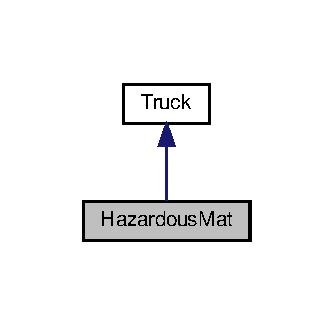
\includegraphics[width=160pt]{class_hazardous_mat__inherit__graph}
\end{center}
\end{figure}


Collaboration diagram for Hazardous\+Mat\+:\nopagebreak
\begin{figure}[H]
\begin{center}
\leavevmode
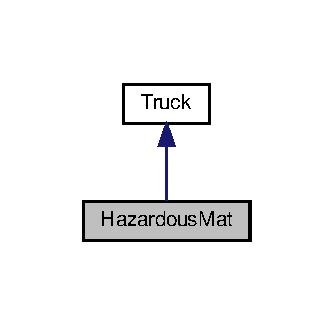
\includegraphics[width=160pt]{class_hazardous_mat__coll__graph}
\end{center}
\end{figure}
\subsection*{Public Member Functions}
\begin{DoxyCompactItemize}
\item 
\hyperlink{class_hazardous_mat_a59551c520358aaae7ed899c2344af6a9}{Hazardous\+Mat} (string license, bool \hyperlink{class_truck_a4189fe5ed32f6084459a9c5ae1eb7c2a}{available}, bool \hyperlink{class_truck_a80b8405cf7a15b236fef70116f99c4fb}{registered}, unsigned short \hyperlink{class_truck_ab004524786ae7aebf7c7bdb5e1599696}{capacity}, unsigned short cargo, car\+\_\+brand \hyperlink{class_truck_a4e30b27a9898eba7ac8404d25cbdd265}{brand})
\begin{DoxyCompactList}\small\item\em constructor for this subclass that calls the one from superclass \end{DoxyCompactList}\item 
\hyperlink{class_hazardous_mat_aa4304419b08381d4aa46d240ca44738a}{$\sim$\+Hazardous\+Mat} ()
\begin{DoxyCompactList}\small\item\em Default destructor. \end{DoxyCompactList}\item 
void \hyperlink{class_hazardous_mat_ab07463da3e9a5d3b8933d2b01332ed00}{info} ()
\begin{DoxyCompactList}\small\item\em Prints more specific information about this truck\textquotesingle{}s subclass. \end{DoxyCompactList}\item 
type \hyperlink{class_hazardous_mat_aed587121cdff185be91ad9ec5ba4d380}{get\+Type} ()
\begin{DoxyCompactList}\small\item\em return type of truck \end{DoxyCompactList}\end{DoxyCompactItemize}
\subsection*{Static Public Attributes}
\begin{DoxyCompactItemize}
\item 
\mbox{\Hypertarget{class_hazardous_mat_a9f71519edca3e72082720686781c34dc}\label{class_hazardous_mat_a9f71519edca3e72082720686781c34dc}} 
static float {\bfseries price\+Per\+KG}
\item 
static unordered\+\_\+map$<$ Hazard\+\_\+enum, float $>$ \hyperlink{class_hazardous_mat_a0d695364bed729ddeca5851314281ad2}{hazard\+Mul}
\item 
static map$<$ unsigned, unsigned $>$ \hyperlink{class_hazardous_mat_a5deebb5a87aa507f2a22065039a3dc2d}{Cap\+Dist}
\end{DoxyCompactItemize}
\subsection*{Additional Inherited Members}


\subsection{Constructor \& Destructor Documentation}
\mbox{\Hypertarget{class_hazardous_mat_a59551c520358aaae7ed899c2344af6a9}\label{class_hazardous_mat_a59551c520358aaae7ed899c2344af6a9}} 
\index{Hazardous\+Mat@{Hazardous\+Mat}!Hazardous\+Mat@{Hazardous\+Mat}}
\index{Hazardous\+Mat@{Hazardous\+Mat}!Hazardous\+Mat@{Hazardous\+Mat}}
\subsubsection{\texorpdfstring{Hazardous\+Mat()}{HazardousMat()}}
{\footnotesize\ttfamily Hazardous\+Mat\+::\+Hazardous\+Mat (\begin{DoxyParamCaption}\item[{string}]{license,  }\item[{bool}]{available,  }\item[{bool}]{registered,  }\item[{unsigned short}]{capacity,  }\item[{unsigned short}]{cargo,  }\item[{car\+\_\+brand}]{brand }\end{DoxyParamCaption})}



constructor for this subclass that calls the one from superclass 

\begin{DoxyReturn}{Returns}
Returns nothing 
\end{DoxyReturn}
\mbox{\Hypertarget{class_hazardous_mat_aa4304419b08381d4aa46d240ca44738a}\label{class_hazardous_mat_aa4304419b08381d4aa46d240ca44738a}} 
\index{Hazardous\+Mat@{Hazardous\+Mat}!````~Hazardous\+Mat@{$\sim$\+Hazardous\+Mat}}
\index{````~Hazardous\+Mat@{$\sim$\+Hazardous\+Mat}!Hazardous\+Mat@{Hazardous\+Mat}}
\subsubsection{\texorpdfstring{$\sim$\+Hazardous\+Mat()}{~HazardousMat()}}
{\footnotesize\ttfamily Hazardous\+Mat\+::$\sim$\+Hazardous\+Mat (\begin{DoxyParamCaption}{ }\end{DoxyParamCaption})\hspace{0.3cm}{\ttfamily [inline]}}



Default destructor. 

\begin{DoxyReturn}{Returns}
Returns nothing 
\end{DoxyReturn}


\subsection{Member Function Documentation}
\mbox{\Hypertarget{class_hazardous_mat_aed587121cdff185be91ad9ec5ba4d380}\label{class_hazardous_mat_aed587121cdff185be91ad9ec5ba4d380}} 
\index{Hazardous\+Mat@{Hazardous\+Mat}!get\+Type@{get\+Type}}
\index{get\+Type@{get\+Type}!Hazardous\+Mat@{Hazardous\+Mat}}
\subsubsection{\texorpdfstring{get\+Type()}{getType()}}
{\footnotesize\ttfamily type Hazardous\+Mat\+::get\+Type (\begin{DoxyParamCaption}{ }\end{DoxyParamCaption})\hspace{0.3cm}{\ttfamily [virtual]}}



return type of truck 

\begin{DoxyReturn}{Returns}
Returns type of truck 
\end{DoxyReturn}


Reimplemented from \hyperlink{class_truck_a24406caf4d09be7f3eff069ce6bc015b}{Truck}.

\mbox{\Hypertarget{class_hazardous_mat_ab07463da3e9a5d3b8933d2b01332ed00}\label{class_hazardous_mat_ab07463da3e9a5d3b8933d2b01332ed00}} 
\index{Hazardous\+Mat@{Hazardous\+Mat}!info@{info}}
\index{info@{info}!Hazardous\+Mat@{Hazardous\+Mat}}
\subsubsection{\texorpdfstring{info()}{info()}}
{\footnotesize\ttfamily void Hazardous\+Mat\+::info (\begin{DoxyParamCaption}{ }\end{DoxyParamCaption})\hspace{0.3cm}{\ttfamily [virtual]}}



Prints more specific information about this truck\textquotesingle{}s subclass. 

\begin{DoxyReturn}{Returns}
Returns nothing 
\end{DoxyReturn}


Reimplemented from \hyperlink{class_truck_a38f09eab2822524e355ecf6d0a13f7de}{Truck}.



\subsection{Member Data Documentation}
\mbox{\Hypertarget{class_hazardous_mat_a5deebb5a87aa507f2a22065039a3dc2d}\label{class_hazardous_mat_a5deebb5a87aa507f2a22065039a3dc2d}} 
\index{Hazardous\+Mat@{Hazardous\+Mat}!Cap\+Dist@{Cap\+Dist}}
\index{Cap\+Dist@{Cap\+Dist}!Hazardous\+Mat@{Hazardous\+Mat}}
\subsubsection{\texorpdfstring{Cap\+Dist}{CapDist}}
{\footnotesize\ttfamily map$<$ unsigned, unsigned $>$ Hazardous\+Mat\+::\+Cap\+Dist\hspace{0.3cm}{\ttfamily [static]}}

holds how many trucks of this have x capacity being that the latter is the key \mbox{\Hypertarget{class_hazardous_mat_a0d695364bed729ddeca5851314281ad2}\label{class_hazardous_mat_a0d695364bed729ddeca5851314281ad2}} 
\index{Hazardous\+Mat@{Hazardous\+Mat}!hazard\+Mul@{hazard\+Mul}}
\index{hazard\+Mul@{hazard\+Mul}!Hazardous\+Mat@{Hazardous\+Mat}}
\subsubsection{\texorpdfstring{hazard\+Mul}{hazardMul}}
{\footnotesize\ttfamily unordered\+\_\+map$<$ Hazard\+\_\+enum, float $>$ Hazardous\+Mat\+::hazard\+Mul\hspace{0.3cm}{\ttfamily [static]}}

will hold price multipliers depending on the service 

The documentation for this class was generated from the following files\+:\begin{DoxyCompactItemize}
\item 
truck.\+h\item 
truck.\+cpp\end{DoxyCompactItemize}

\hypertarget{class_hazardous_service}{}\section{Hazardous\+Service Class Reference}
\label{class_hazardous_service}\index{Hazardous\+Service@{Hazardous\+Service}}


Inheritance diagram for Hazardous\+Service\+:\nopagebreak
\begin{figure}[H]
\begin{center}
\leavevmode
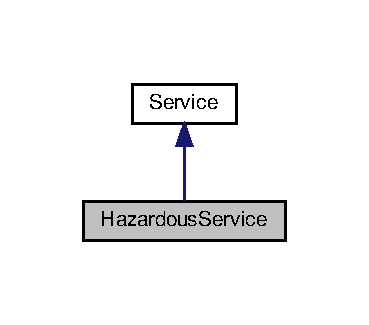
\includegraphics[width=177pt]{class_hazardous_service__inherit__graph}
\end{center}
\end{figure}


Collaboration diagram for Hazardous\+Service\+:
\nopagebreak
\begin{figure}[H]
\begin{center}
\leavevmode
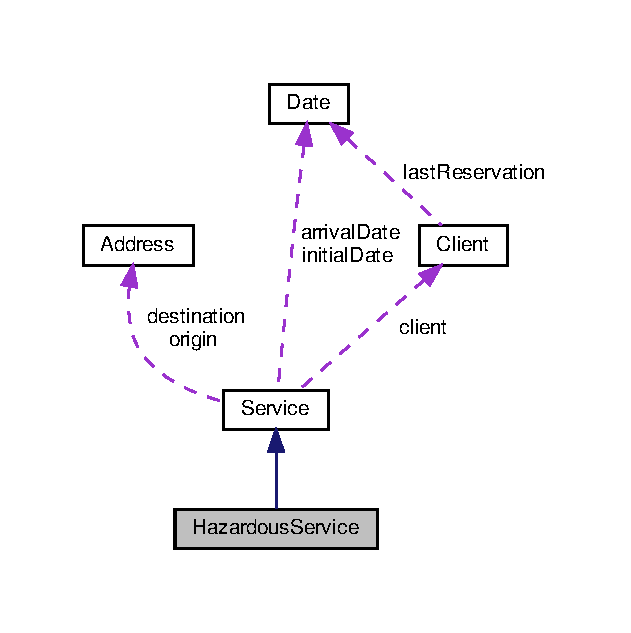
\includegraphics[width=276pt]{class_hazardous_service__coll__graph}
\end{center}
\end{figure}
\subsection*{Public Member Functions}
\begin{DoxyCompactItemize}
\item 
\mbox{\Hypertarget{class_hazardous_service_afcd54cb1f6917720b1845c80e8503827}\label{class_hazardous_service_afcd54cb1f6917720b1845c80e8503827}} 
{\bfseries Hazardous\+Service} (string material, \hyperlink{class_address}{Address} \hyperlink{class_service_a4abd0a104d97e5bdb8e8ca93bab31ce7}{origin}, \hyperlink{class_address}{Address} destination, \hyperlink{class_date}{Date} $\ast$arrival\+Date, unsigned distance, type type, state state, \hyperlink{class_date}{Date} $\ast$date, \hyperlink{class_client}{Client} $\ast$client, float quantity, Hazard\+\_\+enum hazard)
\item 
\mbox{\Hypertarget{class_hazardous_service_af33995d8d0934550a13aa8439c825f9b}\label{class_hazardous_service_af33995d8d0934550a13aa8439c825f9b}} 
{\bfseries Hazardous\+Service} (string material, string \hyperlink{class_service_a4abd0a104d97e5bdb8e8ca93bab31ce7}{origin}, string destination, \hyperlink{class_date}{Date} $\ast$arrival\+Date, unsigned distance, type type, state state, \hyperlink{class_date}{Date} $\ast$date, \hyperlink{class_client}{Client} $\ast$client, float quantity, Hazard\+\_\+enum hazard, float total\+\_\+price, unsigned id)
\end{DoxyCompactItemize}
\subsection*{Public Attributes}
\begin{DoxyCompactItemize}
\item 
\mbox{\Hypertarget{class_hazardous_service_a210252b82d2999d1743d2d695798a555}\label{class_hazardous_service_a210252b82d2999d1743d2d695798a555}} 
Hazard\+\_\+enum {\bfseries type}
\end{DoxyCompactItemize}
\subsection*{Additional Inherited Members}


The documentation for this class was generated from the following file\+:\begin{DoxyCompactItemize}
\item 
service.\+h\end{DoxyCompactItemize}

\hypertarget{class_normal}{}\section{Normal Class Reference}
\label{class_normal}\index{Normal@{Normal}}


Inheritance diagram for Normal\+:\nopagebreak
\begin{figure}[H]
\begin{center}
\leavevmode
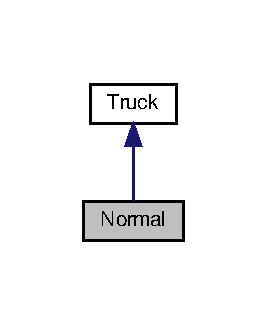
\includegraphics[width=128pt]{class_normal__inherit__graph}
\end{center}
\end{figure}


Collaboration diagram for Normal\+:\nopagebreak
\begin{figure}[H]
\begin{center}
\leavevmode
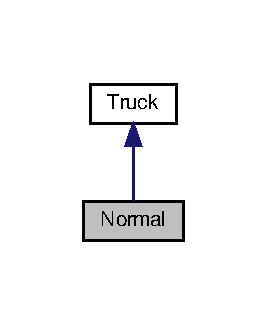
\includegraphics[width=128pt]{class_normal__coll__graph}
\end{center}
\end{figure}
\subsection*{Public Member Functions}
\begin{DoxyCompactItemize}
\item 
\hyperlink{class_normal_a5bfcd1d763c6cf56bdcf4de370903da7}{Normal} (string license, bool \hyperlink{class_truck_a4189fe5ed32f6084459a9c5ae1eb7c2a}{available}, bool \hyperlink{class_truck_a80b8405cf7a15b236fef70116f99c4fb}{registered}, unsigned short \hyperlink{class_truck_ab004524786ae7aebf7c7bdb5e1599696}{capacity}, unsigned short cargo)
\begin{DoxyCompactList}\small\item\em constructor for this subclass that calls the one from superclass \end{DoxyCompactList}\item 
\hyperlink{class_normal_a2ed547e3b7361c3675224d352cf79740}{$\sim$\+Normal} ()
\begin{DoxyCompactList}\small\item\em Default destructor. \end{DoxyCompactList}\item 
void \hyperlink{class_normal_ade6add2ee09e701113534c97e2a03307}{info} ()
\begin{DoxyCompactList}\small\item\em Prints more specific information about this truck\textquotesingle{}s subclass. \end{DoxyCompactList}\item 
type \hyperlink{class_normal_ae34be8332ea67df5fb0ae9b274884748}{get\+Type} ()
\begin{DoxyCompactList}\small\item\em return type of truck \end{DoxyCompactList}\end{DoxyCompactItemize}
\subsection*{Static Public Attributes}
\begin{DoxyCompactItemize}
\item 
\mbox{\Hypertarget{class_normal_a8aae6212077e4f0c359d7fcfb5af3743}\label{class_normal_a8aae6212077e4f0c359d7fcfb5af3743}} 
static float {\bfseries price\+Per\+KG}
\item 
static map$<$ unsigned, unsigned $>$ \hyperlink{class_normal_a1ccae0db66db16a387c05009bf7194f8}{Cap\+Dist}
\end{DoxyCompactItemize}
\subsection*{Additional Inherited Members}


\subsection{Constructor \& Destructor Documentation}
\mbox{\Hypertarget{class_normal_a5bfcd1d763c6cf56bdcf4de370903da7}\label{class_normal_a5bfcd1d763c6cf56bdcf4de370903da7}} 
\index{Normal@{Normal}!Normal@{Normal}}
\index{Normal@{Normal}!Normal@{Normal}}
\subsubsection{\texorpdfstring{Normal()}{Normal()}}
{\footnotesize\ttfamily Normal\+::\+Normal (\begin{DoxyParamCaption}\item[{string}]{license,  }\item[{bool}]{available,  }\item[{bool}]{registered,  }\item[{unsigned short}]{capacity,  }\item[{unsigned short}]{cargo }\end{DoxyParamCaption})}



constructor for this subclass that calls the one from superclass 

\begin{DoxyReturn}{Returns}
Returns nothing 
\end{DoxyReturn}
\mbox{\Hypertarget{class_normal_a2ed547e3b7361c3675224d352cf79740}\label{class_normal_a2ed547e3b7361c3675224d352cf79740}} 
\index{Normal@{Normal}!````~Normal@{$\sim$\+Normal}}
\index{````~Normal@{$\sim$\+Normal}!Normal@{Normal}}
\subsubsection{\texorpdfstring{$\sim$\+Normal()}{~Normal()}}
{\footnotesize\ttfamily Normal\+::$\sim$\+Normal (\begin{DoxyParamCaption}{ }\end{DoxyParamCaption})\hspace{0.3cm}{\ttfamily [inline]}}



Default destructor. 

\begin{DoxyReturn}{Returns}
Returns nothing 
\end{DoxyReturn}


\subsection{Member Function Documentation}
\mbox{\Hypertarget{class_normal_ae34be8332ea67df5fb0ae9b274884748}\label{class_normal_ae34be8332ea67df5fb0ae9b274884748}} 
\index{Normal@{Normal}!get\+Type@{get\+Type}}
\index{get\+Type@{get\+Type}!Normal@{Normal}}
\subsubsection{\texorpdfstring{get\+Type()}{getType()}}
{\footnotesize\ttfamily type Normal\+::get\+Type (\begin{DoxyParamCaption}{ }\end{DoxyParamCaption})\hspace{0.3cm}{\ttfamily [virtual]}}



return type of truck 

\begin{DoxyReturn}{Returns}
Returns type of truck 
\end{DoxyReturn}


Reimplemented from \hyperlink{class_truck_a24406caf4d09be7f3eff069ce6bc015b}{Truck}.

\mbox{\Hypertarget{class_normal_ade6add2ee09e701113534c97e2a03307}\label{class_normal_ade6add2ee09e701113534c97e2a03307}} 
\index{Normal@{Normal}!info@{info}}
\index{info@{info}!Normal@{Normal}}
\subsubsection{\texorpdfstring{info()}{info()}}
{\footnotesize\ttfamily void Normal\+::info (\begin{DoxyParamCaption}{ }\end{DoxyParamCaption})\hspace{0.3cm}{\ttfamily [virtual]}}



Prints more specific information about this truck\textquotesingle{}s subclass. 

\begin{DoxyReturn}{Returns}
Returns nothing 
\end{DoxyReturn}


Reimplemented from \hyperlink{class_truck_a38f09eab2822524e355ecf6d0a13f7de}{Truck}.



\subsection{Member Data Documentation}
\mbox{\Hypertarget{class_normal_a1ccae0db66db16a387c05009bf7194f8}\label{class_normal_a1ccae0db66db16a387c05009bf7194f8}} 
\index{Normal@{Normal}!Cap\+Dist@{Cap\+Dist}}
\index{Cap\+Dist@{Cap\+Dist}!Normal@{Normal}}
\subsubsection{\texorpdfstring{Cap\+Dist}{CapDist}}
{\footnotesize\ttfamily map$<$ unsigned, unsigned $>$ Normal\+::\+Cap\+Dist\hspace{0.3cm}{\ttfamily [static]}}

holds how many trucks of this have x capacity being that the latter is the key 

The documentation for this class was generated from the following files\+:\begin{DoxyCompactItemize}
\item 
truck.\+h\item 
truck.\+cpp\end{DoxyCompactItemize}

\hypertarget{class_not_a_client}{}\section{Not\+A\+Client Class Reference}
\label{class_not_a_client}\index{Not\+A\+Client@{Not\+A\+Client}}


Inheritance diagram for Not\+A\+Client\+:\nopagebreak
\begin{figure}[H]
\begin{center}
\leavevmode
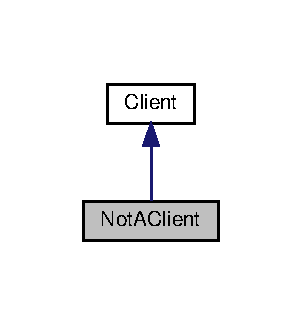
\includegraphics[width=145pt]{class_not_a_client__inherit__graph}
\end{center}
\end{figure}


Collaboration diagram for Not\+A\+Client\+:\nopagebreak
\begin{figure}[H]
\begin{center}
\leavevmode
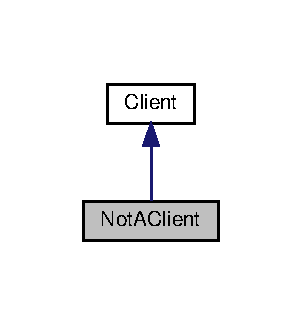
\includegraphics[width=145pt]{class_not_a_client__coll__graph}
\end{center}
\end{figure}
\subsection*{Public Member Functions}
\begin{DoxyCompactItemize}
\item 
\mbox{\Hypertarget{class_not_a_client_ababe63b9416f4dd90045d6086292724d}\label{class_not_a_client_ababe63b9416f4dd90045d6086292724d}} 
{\bfseries Not\+A\+Client} (unsigned nif\+\_\+n, string erro)
\item 
\mbox{\Hypertarget{class_not_a_client_a70136e2a67ce191dd0091bb8ace19dd9}\label{class_not_a_client_a70136e2a67ce191dd0091bb8ace19dd9}} 
unsigned int {\bfseries get\+Nif} () const
\end{DoxyCompactItemize}
\subsection*{Public Attributes}
\begin{DoxyCompactItemize}
\item 
\mbox{\Hypertarget{class_not_a_client_a5a7444300559fedd328e401de04fff79}\label{class_not_a_client_a5a7444300559fedd328e401de04fff79}} 
string {\bfseries erro}
\end{DoxyCompactItemize}
\subsection*{Additional Inherited Members}


The documentation for this class was generated from the following files\+:\begin{DoxyCompactItemize}
\item 
client.\+h\item 
client.\+cpp\end{DoxyCompactItemize}

\hypertarget{class_not_a_truck}{}\section{Not\+A\+Truck Class Reference}
\label{class_not_a_truck}\index{Not\+A\+Truck@{Not\+A\+Truck}}
\subsection*{Public Member Functions}
\begin{DoxyCompactItemize}
\item 
\hyperlink{class_not_a_truck_a52293d9e122db41dc3ff34d5e1019866}{Not\+A\+Truck} (string erro, string license)
\begin{DoxyCompactList}\small\item\em Constructor with all data necessary. \end{DoxyCompactList}\end{DoxyCompactItemize}
\subsection*{Public Attributes}
\begin{DoxyCompactItemize}
\item 
\mbox{\Hypertarget{class_not_a_truck_ac9ff6b8470d3130eb3754f25dd97da72}\label{class_not_a_truck_ac9ff6b8470d3130eb3754f25dd97da72}} 
string {\bfseries erro}
\item 
\mbox{\Hypertarget{class_not_a_truck_a274aa2458fcec7142ebff06fd23a10dc}\label{class_not_a_truck_a274aa2458fcec7142ebff06fd23a10dc}} 
string {\bfseries license}
\end{DoxyCompactItemize}


\subsection{Constructor \& Destructor Documentation}
\mbox{\Hypertarget{class_not_a_truck_a52293d9e122db41dc3ff34d5e1019866}\label{class_not_a_truck_a52293d9e122db41dc3ff34d5e1019866}} 
\index{Not\+A\+Truck@{Not\+A\+Truck}!Not\+A\+Truck@{Not\+A\+Truck}}
\index{Not\+A\+Truck@{Not\+A\+Truck}!Not\+A\+Truck@{Not\+A\+Truck}}
\subsubsection{\texorpdfstring{Not\+A\+Truck()}{NotATruck()}}
{\footnotesize\ttfamily Not\+A\+Truck\+::\+Not\+A\+Truck (\begin{DoxyParamCaption}\item[{string}]{erro,  }\item[{string}]{license }\end{DoxyParamCaption})\hspace{0.3cm}{\ttfamily [inline]}}



Constructor with all data necessary. 

This exception is thrown if the truck is not valid


\begin{DoxyParams}{Parameters}
{\em erro} & -\/ Message describing error \\
\hline
{\em license} & -\/ license that isn\textquotesingle{}t valid \\
\hline
\end{DoxyParams}


The documentation for this class was generated from the following file\+:\begin{DoxyCompactItemize}
\item 
truck.\+h\end{DoxyCompactItemize}

\hypertarget{class_service}{}\section{Service Class Reference}
\label{class_service}\index{Service@{Service}}


Inheritance diagram for Service\+:\nopagebreak
\begin{figure}[H]
\begin{center}
\leavevmode
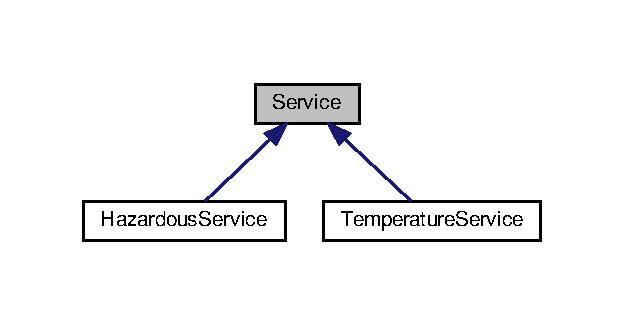
\includegraphics[width=300pt]{class_service__inherit__graph}
\end{center}
\end{figure}


Collaboration diagram for Service\+:
\nopagebreak
\begin{figure}[H]
\begin{center}
\leavevmode
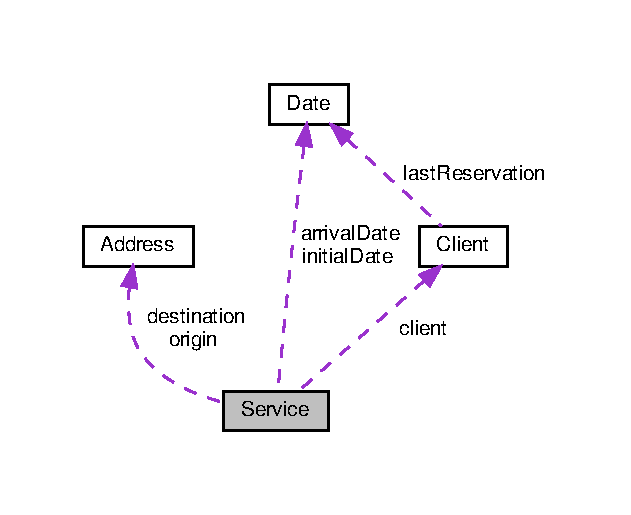
\includegraphics[width=276pt]{class_service__coll__graph}
\end{center}
\end{figure}
\subsection*{Public Member Functions}
\begin{DoxyCompactItemize}
\item 
\hyperlink{class_address}{Address} \hyperlink{class_service_a186e0115cc0197181b4e060bfe4cd502}{get\+Origin} () const
\item 
\mbox{\Hypertarget{class_service_a2aabf308bd77e1de07afa28d5ff72b08}\label{class_service_a2aabf308bd77e1de07afa28d5ff72b08}} 
\hyperlink{class_address}{Address} {\bfseries get\+Destination} () const
\item 
\mbox{\Hypertarget{class_service_a7b36594e1a24656f065f7d41b79bb718}\label{class_service_a7b36594e1a24656f065f7d41b79bb718}} 
unsigned {\bfseries get\+Distance} () const
\item 
\mbox{\Hypertarget{class_service_a75f96cd94a42b604ff179343576e1bba}\label{class_service_a75f96cd94a42b604ff179343576e1bba}} 
type {\bfseries get\+Type} () const
\item 
\mbox{\Hypertarget{class_service_a5a19731d4fa91658afe908167fe66ad6}\label{class_service_a5a19731d4fa91658afe908167fe66ad6}} 
unsigned int {\bfseries get\+Id} () const
\item 
\mbox{\Hypertarget{class_service_adf7f337e38c8de87e82b42f15c7ccad3}\label{class_service_adf7f337e38c8de87e82b42f15c7ccad3}} 
state {\bfseries get\+State} () const
\item 
\mbox{\Hypertarget{class_service_a3a8b665eff7933227303dc070bb29485}\label{class_service_a3a8b665eff7933227303dc070bb29485}} 
\hyperlink{class_date}{Date} $\ast$ {\bfseries get\+I\+Date} () const
\item 
\mbox{\Hypertarget{class_service_a2b08c3d53ab2246eb3cca649c2baa100}\label{class_service_a2b08c3d53ab2246eb3cca649c2baa100}} 
\hyperlink{class_date}{Date} $\ast$ {\bfseries get\+A\+Date} () const
\item 
\mbox{\Hypertarget{class_service_a4a9cc0a45f030f69b3d6468df5d02aaa}\label{class_service_a4a9cc0a45f030f69b3d6468df5d02aaa}} 
\hyperlink{class_client}{Client} $\ast$ {\bfseries get\+Client} () const
\item 
\mbox{\Hypertarget{class_service_a5d4a097657f1cce3b60ab805fbfb0c80}\label{class_service_a5d4a097657f1cce3b60ab805fbfb0c80}} 
vector$<$ \hyperlink{class_truck}{Truck} $\ast$ $>$ $\ast$ {\bfseries get\+Trucks} ()
\item 
\mbox{\Hypertarget{class_service_ac5dca2c1b78ff990827554d4ac9c5990}\label{class_service_ac5dca2c1b78ff990827554d4ac9c5990}} 
float {\bfseries get\+Total\+Price} () const
\item 
\mbox{\Hypertarget{class_service_aceff76eb1aba00c9c74eb98d56771a6a}\label{class_service_aceff76eb1aba00c9c74eb98d56771a6a}} 
float {\bfseries get\+Quantity} () const
\item 
\mbox{\Hypertarget{class_service_a924ea5df81fa28e96b5ef02bad0d6d7f}\label{class_service_a924ea5df81fa28e96b5ef02bad0d6d7f}} 
float {\bfseries get\+Multiplier} ()
\item 
\mbox{\Hypertarget{class_service_a92be216e9c710b28bc4046353884b3e2}\label{class_service_a92be216e9c710b28bc4046353884b3e2}} 
string {\bfseries get\+Material} () const
\item 
\mbox{\Hypertarget{class_service_af3f248b1ecea5fd3fb0da198bfdbc7d5}\label{class_service_af3f248b1ecea5fd3fb0da198bfdbc7d5}} 
void {\bfseries set\+Origin} (\hyperlink{class_address}{Address} \hyperlink{class_service_a4abd0a104d97e5bdb8e8ca93bab31ce7}{origin})
\item 
\mbox{\Hypertarget{class_service_a1c2082379deaf672919165e540afcab2}\label{class_service_a1c2082379deaf672919165e540afcab2}} 
void {\bfseries set\+Destination} (\hyperlink{class_address}{Address} destination)
\item 
\mbox{\Hypertarget{class_service_aed76805ea044b29f0dafe65a7d39f2dc}\label{class_service_aed76805ea044b29f0dafe65a7d39f2dc}} 
void {\bfseries set\+Time} (double time)
\item 
\mbox{\Hypertarget{class_service_a6349774a4ab8afffe88dc51025690650}\label{class_service_a6349774a4ab8afffe88dc51025690650}} 
void {\bfseries set\+Distance} (unsigned distance)
\item 
\mbox{\Hypertarget{class_service_af26945add8ad6504432fa0c62c8c2769}\label{class_service_af26945add8ad6504432fa0c62c8c2769}} 
void {\bfseries set\+Type} (type type)
\item 
\mbox{\Hypertarget{class_service_a7aa57d557be113ce2025843cb1046137}\label{class_service_a7aa57d557be113ce2025843cb1046137}} 
void {\bfseries set\+State} (state state)
\item 
\mbox{\Hypertarget{class_service_ac4635d11b13279a4ef84b1c6378639d4}\label{class_service_ac4635d11b13279a4ef84b1c6378639d4}} 
void {\bfseries set\+I\+Date} (\hyperlink{class_date}{Date} $\ast$date)
\item 
\mbox{\Hypertarget{class_service_a80210953169ca04d454db8be48694187}\label{class_service_a80210953169ca04d454db8be48694187}} 
void {\bfseries set\+A\+Date} (\hyperlink{class_date}{Date} $\ast$date)
\item 
\mbox{\Hypertarget{class_service_a1cf3d0b85e44bd7ec58e4a12a7432aef}\label{class_service_a1cf3d0b85e44bd7ec58e4a12a7432aef}} 
void {\bfseries set\+Client} (\hyperlink{class_client}{Client} $\ast$client)
\item 
\mbox{\Hypertarget{class_service_a29386f4e82e1de1f654468d4a020c6a4}\label{class_service_a29386f4e82e1de1f654468d4a020c6a4}} 
void {\bfseries set\+Quantity} (float quantity)
\item 
\mbox{\Hypertarget{class_service_a9fcafc3bcbdc0b436860ee5626c69ce1}\label{class_service_a9fcafc3bcbdc0b436860ee5626c69ce1}} 
void {\bfseries set\+Material} (string material)
\item 
\mbox{\Hypertarget{class_service_aa6203cff9343cb8e7bf996514f14179d}\label{class_service_aa6203cff9343cb8e7bf996514f14179d}} 
void {\bfseries add\+Truck} (\hyperlink{class_truck}{Truck} $\ast$truck)
\item 
\mbox{\Hypertarget{class_service_a9efe3e195062d8f668e49be1759d325c}\label{class_service_a9efe3e195062d8f668e49be1759d325c}} 
void {\bfseries calc\+Price} ()
\item 
\mbox{\Hypertarget{class_service_a351a27eebc07d1ff3f433d6ad356925a}\label{class_service_a351a27eebc07d1ff3f433d6ad356925a}} 
void {\bfseries edit\+Service} ()
\end{DoxyCompactItemize}
\subsection*{Static Public Member Functions}
\begin{DoxyCompactItemize}
\item 
\mbox{\Hypertarget{class_service_aa3672a3a070ca951f5b66075a5d4c339}\label{class_service_aa3672a3a070ca951f5b66075a5d4c339}} 
static void {\bfseries save\+To\+File} (list$<$ \hyperlink{class_service}{Service} $\ast$$>$ $\ast$services\+\_\+finished, vector$<$ \hyperlink{class_service}{Service} $\ast$$>$ $\ast$services\+\_\+on\+\_\+transit, vector$<$ \hyperlink{class_service}{Service} $\ast$$>$ $\ast$services\+\_\+on\+\_\+queue)
\item 
\mbox{\Hypertarget{class_service_add72b2a9e781bdb20a26bdff39952088}\label{class_service_add72b2a9e781bdb20a26bdff39952088}} 
static void {\bfseries load\+From\+File} (list$<$ \hyperlink{class_service}{Service} $\ast$$>$ $\ast$services\+\_\+finished, vector$<$ \hyperlink{class_service}{Service} $\ast$$>$ $\ast$services\+\_\+on\+\_\+transit, vector$<$ \hyperlink{class_service}{Service} $\ast$$>$ $\ast$services\+\_\+on\+\_\+queue)
\item 
\mbox{\Hypertarget{class_service_a9e1aa933d52a23d5e265666bdedea0f1}\label{class_service_a9e1aa933d52a23d5e265666bdedea0f1}} 
static \hyperlink{class_service}{Service} $\ast$ {\bfseries add\+Service} (vector$<$ \hyperlink{class_service}{Service} $\ast$$>$ $\ast$services, \hyperlink{class_client}{Client} $\ast$client=nullptr)
\item 
\mbox{\Hypertarget{class_service_af2ca48ced14708abeb5f92f10245241c}\label{class_service_af2ca48ced14708abeb5f92f10245241c}} 
static bool {\bfseries remove\+Service} (vector$<$ \hyperlink{class_service}{Service} $\ast$$>$ $\ast$services, unsigned id)
\end{DoxyCompactItemize}
\subsection*{Protected Member Functions}
\begin{DoxyCompactItemize}
\item 
\mbox{\Hypertarget{class_service_ab00ec0b62c00dc5dfad8442c85de3b12}\label{class_service_ab00ec0b62c00dc5dfad8442c85de3b12}} 
{\bfseries Service} (string material, \hyperlink{class_address}{Address} \hyperlink{class_service_a4abd0a104d97e5bdb8e8ca93bab31ce7}{origin}, \hyperlink{class_address}{Address} destination, \hyperlink{class_date}{Date} $\ast$arrival\+Date, unsigned distance, type type, state state, \hyperlink{class_date}{Date} $\ast$date, \hyperlink{class_client}{Client} $\ast$client, float quantity)
\item 
\mbox{\Hypertarget{class_service_aa8037c739c084ca5f12d25de6316d5ca}\label{class_service_aa8037c739c084ca5f12d25de6316d5ca}} 
{\bfseries Service} (string material, string \hyperlink{class_service_a4abd0a104d97e5bdb8e8ca93bab31ce7}{origin}, string destination, \hyperlink{class_date}{Date} $\ast$arrival\+Date, unsigned distance, type type, state state, \hyperlink{class_date}{Date} $\ast$date, \hyperlink{class_client}{Client} $\ast$client, float quantity, float total\+\_\+price, unsigned id)
\end{DoxyCompactItemize}
\subsection*{Protected Attributes}
\begin{DoxyCompactItemize}
\item 
\hyperlink{class_address}{Address} $\ast$ \hyperlink{class_service_a4abd0a104d97e5bdb8e8ca93bab31ce7}{origin}
\item 
\mbox{\Hypertarget{class_service_adf346b71b98618cf84e5d0a0eca2ee1e}\label{class_service_adf346b71b98618cf84e5d0a0eca2ee1e}} 
\hyperlink{class_address}{Address} $\ast$ {\bfseries destination}
\item 
\mbox{\Hypertarget{class_service_a04a4efb2434d7c4acb7c43bfef2d9c52}\label{class_service_a04a4efb2434d7c4acb7c43bfef2d9c52}} 
string {\bfseries material}
\item 
\mbox{\Hypertarget{class_service_a1e1bdf965c61c9d52c6992beb5594032}\label{class_service_a1e1bdf965c61c9d52c6992beb5594032}} 
\hyperlink{class_date}{Date} $\ast$ {\bfseries arrival\+Date}
\item 
\mbox{\Hypertarget{class_service_ad183cae7d3eeb78860669d209f4e7387}\label{class_service_ad183cae7d3eeb78860669d209f4e7387}} 
unsigned {\bfseries distance}
\item 
\mbox{\Hypertarget{class_service_afef38ab183af6a2b6fba08400c9eb987}\label{class_service_afef38ab183af6a2b6fba08400c9eb987}} 
float {\bfseries quantity}
\item 
\mbox{\Hypertarget{class_service_acb458e8692722cfba06273fb938c2bf8}\label{class_service_acb458e8692722cfba06273fb938c2bf8}} 
type {\bfseries ser\+\_\+type}
\item 
\mbox{\Hypertarget{class_service_adae62762a30190e27f24e40c7dbebae5}\label{class_service_adae62762a30190e27f24e40c7dbebae5}} 
unsigned int {\bfseries id}
\item 
\mbox{\Hypertarget{class_service_a179356d0a67dfff27fb9417db0c9357b}\label{class_service_a179356d0a67dfff27fb9417db0c9357b}} 
vector$<$ \hyperlink{class_truck}{Truck} $\ast$ $>$ {\bfseries trucks}
\item 
\mbox{\Hypertarget{class_service_ae0321f4e4847e9e413910831262c89c4}\label{class_service_ae0321f4e4847e9e413910831262c89c4}} 
state {\bfseries ser\+\_\+state}
\item 
\mbox{\Hypertarget{class_service_a16f7facc8c1f9dd5ad1a58750e20aea1}\label{class_service_a16f7facc8c1f9dd5ad1a58750e20aea1}} 
\hyperlink{class_date}{Date} $\ast$ {\bfseries initial\+Date}
\item 
\mbox{\Hypertarget{class_service_ac7249f01861124261b7b4b23bb27ab3e}\label{class_service_ac7249f01861124261b7b4b23bb27ab3e}} 
\hyperlink{class_client}{Client} $\ast$ {\bfseries client}
\item 
\mbox{\Hypertarget{class_service_a9aad689e8f65b495425fda35cf5662ed}\label{class_service_a9aad689e8f65b495425fda35cf5662ed}} 
float {\bfseries total\+\_\+price}
\end{DoxyCompactItemize}
\subsection*{Static Protected Attributes}
\begin{DoxyCompactItemize}
\item 
\mbox{\Hypertarget{class_service_aa80a6461b0877972c7bbd427cff39175}\label{class_service_aa80a6461b0877972c7bbd427cff39175}} 
static unsigned int {\bfseries last\+Id} =0
\end{DoxyCompactItemize}
\subsection*{Friends}
\begin{DoxyCompactItemize}
\item 
\mbox{\Hypertarget{class_service_a641fd7efe1dd35ea19ac062c4e2ece45}\label{class_service_a641fd7efe1dd35ea19ac062c4e2ece45}} 
ostream \& {\bfseries operator$<$$<$} (ostream \&os, \hyperlink{class_service}{Service} $\ast$a)
\end{DoxyCompactItemize}


\subsection{Member Function Documentation}
\mbox{\Hypertarget{class_service_a186e0115cc0197181b4e060bfe4cd502}\label{class_service_a186e0115cc0197181b4e060bfe4cd502}} 
\index{Service@{Service}!get\+Origin@{get\+Origin}}
\index{get\+Origin@{get\+Origin}!Service@{Service}}
\subsubsection{\texorpdfstring{get\+Origin()}{getOrigin()}}
{\footnotesize\ttfamily \hyperlink{class_address}{Address} Service\+::get\+Origin (\begin{DoxyParamCaption}{ }\end{DoxyParamCaption}) const}

\begin{DoxyReturn}{Returns}
string \hyperlink{class_service_a4abd0a104d97e5bdb8e8ca93bab31ce7}{origin} 
\end{DoxyReturn}


\subsection{Member Data Documentation}
\mbox{\Hypertarget{class_service_a4abd0a104d97e5bdb8e8ca93bab31ce7}\label{class_service_a4abd0a104d97e5bdb8e8ca93bab31ce7}} 
\index{Service@{Service}!origin@{origin}}
\index{origin@{origin}!Service@{Service}}
\subsubsection{\texorpdfstring{origin}{origin}}
{\footnotesize\ttfamily \hyperlink{class_address}{Address}$\ast$ Service\+::origin\hspace{0.3cm}{\ttfamily [protected]}}

stores the origin of the \hyperlink{class_service}{Service} 

The documentation for this class was generated from the following files\+:\begin{DoxyCompactItemize}
\item 
service.\+h\item 
service.\+cpp\end{DoxyCompactItemize}

\hypertarget{class_service_do_not_exist}{}\section{Service\+Do\+Not\+Exist Class Reference}
\label{class_service_do_not_exist}\index{Service\+Do\+Not\+Exist@{Service\+Do\+Not\+Exist}}


Constructor with all data necessary.  




{\ttfamily \#include $<$service.\+h$>$}

\subsection*{Public Member Functions}
\begin{DoxyCompactItemize}
\item 
\mbox{\Hypertarget{class_service_do_not_exist_a972a9da7853eb19d42c57b8661bbbe9d}\label{class_service_do_not_exist_a972a9da7853eb19d42c57b8661bbbe9d}} 
{\bfseries Service\+Do\+Not\+Exist} (string erro)
\end{DoxyCompactItemize}
\subsection*{Public Attributes}
\begin{DoxyCompactItemize}
\item 
\mbox{\Hypertarget{class_service_do_not_exist_a8915a28a1a9b0f2c85a411be65b34c91}\label{class_service_do_not_exist_a8915a28a1a9b0f2c85a411be65b34c91}} 
string {\bfseries erro}
\end{DoxyCompactItemize}


\subsection{Detailed Description}
Constructor with all data necessary. 

This exception is thrown if the program is unable to find a service


\begin{DoxyParams}{Parameters}
{\em erro} & -\/ Message describing error \\
\hline
\end{DoxyParams}


The documentation for this class was generated from the following file\+:\begin{DoxyCompactItemize}
\item 
service.\+h\end{DoxyCompactItemize}

\hypertarget{class_temperature_service}{}\section{Temperature\+Service Class Reference}
\label{class_temperature_service}\index{Temperature\+Service@{Temperature\+Service}}


Inheritance diagram for Temperature\+Service\+:\nopagebreak
\begin{figure}[H]
\begin{center}
\leavevmode
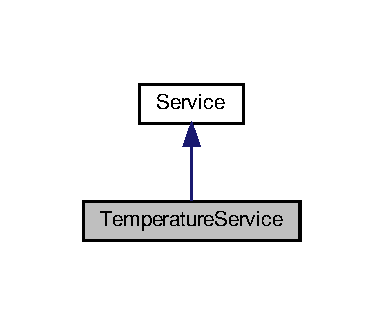
\includegraphics[width=184pt]{class_temperature_service__inherit__graph}
\end{center}
\end{figure}


Collaboration diagram for Temperature\+Service\+:\nopagebreak
\begin{figure}[H]
\begin{center}
\leavevmode
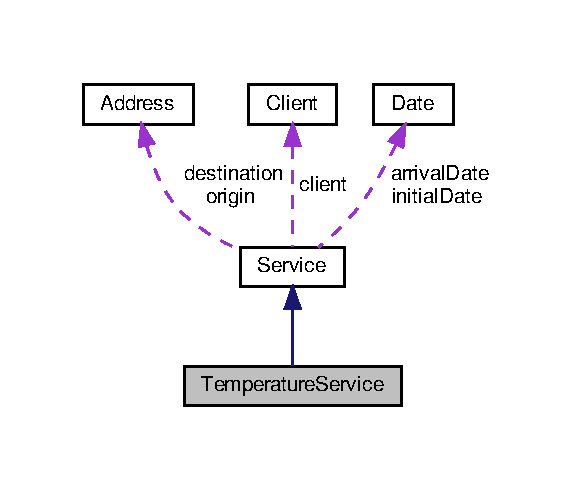
\includegraphics[width=200pt]{class_temperature_service__coll__graph}
\end{center}
\end{figure}
\subsection*{Public Member Functions}
\begin{DoxyCompactItemize}
\item 
\mbox{\Hypertarget{class_temperature_service_a94888d7ca82463249929415a135f1264}\label{class_temperature_service_a94888d7ca82463249929415a135f1264}} 
{\bfseries Temperature\+Service} (string material, string \hyperlink{class_service_a0e23ac4930720ab597a5c584703151f9}{origin}, string destination, \hyperlink{class_date}{Date} $\ast$arrival\+Date, unsigned distance, type type, state state, \hyperlink{class_date}{Date} $\ast$date, \hyperlink{class_client}{Client} $\ast$client, float quantity, Temperature\+\_\+enum hazard)
\item 
\mbox{\Hypertarget{class_temperature_service_a980fd4745f1dc221fee79bff5f126ad5}\label{class_temperature_service_a980fd4745f1dc221fee79bff5f126ad5}} 
{\bfseries Temperature\+Service} (string material, string \hyperlink{class_service_a0e23ac4930720ab597a5c584703151f9}{origin}, string destination, \hyperlink{class_date}{Date} $\ast$arrival\+Date, unsigned distance, type type, state state, \hyperlink{class_date}{Date} $\ast$date, \hyperlink{class_client}{Client} $\ast$client, float quantity, Temperature\+\_\+enum hazard, float total\+\_\+price, unsigned id\+\_\+s)
\end{DoxyCompactItemize}
\subsection*{Public Attributes}
\begin{DoxyCompactItemize}
\item 
\mbox{\Hypertarget{class_temperature_service_a1c6c01171d9ad6e56012440fb85a17bd}\label{class_temperature_service_a1c6c01171d9ad6e56012440fb85a17bd}} 
Temperature\+\_\+enum {\bfseries type}
\end{DoxyCompactItemize}
\subsection*{Additional Inherited Members}


The documentation for this class was generated from the following file\+:\begin{DoxyCompactItemize}
\item 
service.\+h\end{DoxyCompactItemize}

\hypertarget{class_truck}{}\section{Truck Class Reference}
\label{class_truck}\index{Truck@{Truck}}


Inheritance diagram for Truck\+:\nopagebreak
\begin{figure}[H]
\begin{center}
\leavevmode
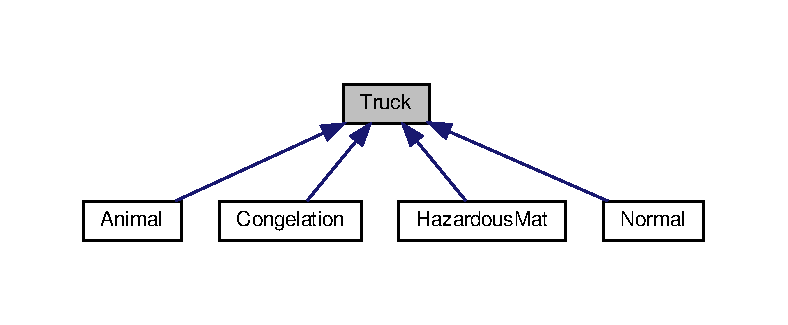
\includegraphics[width=350pt]{class_truck__inherit__graph}
\end{center}
\end{figure}
\subsection*{Public Member Functions}
\begin{DoxyCompactItemize}
\item 
\mbox{\Hypertarget{class_truck_a310563b5c12feb94c1e1f8f855c1ee05}\label{class_truck_a310563b5c12feb94c1e1f8f855c1ee05}} 
\hyperlink{class_truck_a310563b5c12feb94c1e1f8f855c1ee05}{Truck} (string license, bool available, bool \hyperlink{class_truck_a80b8405cf7a15b236fef70116f99c4fb}{registered}, unsigned short \hyperlink{class_truck_a14541fad6d47c606ce4e1bd150a68a23}{capacity}, unsigned short \hyperlink{class_truck_a968fc6b1a6171a03e4254d6615da4ecd}{cargo})
\begin{DoxyCompactList}\small\item\em if in transit this holds the weight it transports, if not it is 0 \end{DoxyCompactList}\item 
\mbox{\Hypertarget{class_truck_ad775a01ae4cb8c36d6e2438f4dd37792}\label{class_truck_ad775a01ae4cb8c36d6e2438f4dd37792}} 
unsigned short {\bfseries getcapacity} () const
\item 
\mbox{\Hypertarget{class_truck_a0eaa329bc72bf0171f7ec2a0a6240156}\label{class_truck_a0eaa329bc72bf0171f7ec2a0a6240156}} 
bool {\bfseries getavailable} () const
\item 
\mbox{\Hypertarget{class_truck_ae76a7ae2343557680ae915c6c6d42ff8}\label{class_truck_ae76a7ae2343557680ae915c6c6d42ff8}} 
string {\bfseries getlicense} () const
\item 
\mbox{\Hypertarget{class_truck_a830838ed22465cf27f56b911c3fadf13}\label{class_truck_a830838ed22465cf27f56b911c3fadf13}} 
bool {\bfseries getregistered} () const
\item 
\mbox{\Hypertarget{class_truck_a1bc18daed6fb7f0b900dac32013a250f}\label{class_truck_a1bc18daed6fb7f0b900dac32013a250f}} 
unsigned short {\bfseries getcargo} () const
\item 
\mbox{\Hypertarget{class_truck_a207506f38e78d7a5f065893295a2c00d}\label{class_truck_a207506f38e78d7a5f065893295a2c00d}} 
vector$<$ \hyperlink{class_service}{Service} $\ast$ $>$ $\ast$ {\bfseries get\+Services} ()
\item 
\mbox{\Hypertarget{class_truck_a22d2dc22b1c5b9652d463ec624442403}\label{class_truck_a22d2dc22b1c5b9652d463ec624442403}} 
virtual void {\bfseries setprice} (float newval)
\item 
\mbox{\Hypertarget{class_truck_a9268e17e1a967d1702b28c6940403aa4}\label{class_truck_a9268e17e1a967d1702b28c6940403aa4}} 
void {\bfseries setregistered} (bool foo)
\item 
\mbox{\Hypertarget{class_truck_a59ca935a364da118131ed85647aa4f0d}\label{class_truck_a59ca935a364da118131ed85647aa4f0d}} 
void {\bfseries setavailable} (bool foo)
\item 
\mbox{\Hypertarget{class_truck_a38f09eab2822524e355ecf6d0a13f7de}\label{class_truck_a38f09eab2822524e355ecf6d0a13f7de}} 
virtual void {\bfseries info} ()
\item 
\mbox{\Hypertarget{class_truck_a03c8acd51c35f24db74cd8b2ee20cacb}\label{class_truck_a03c8acd51c35f24db74cd8b2ee20cacb}} 
void {\bfseries add\+\_\+service} (\hyperlink{class_service}{Service} $\ast$service)
\item 
\mbox{\Hypertarget{class_truck_a0abc7397fd6dba0eeeb2b5ae3e225fd1}\label{class_truck_a0abc7397fd6dba0eeeb2b5ae3e225fd1}} 
void {\bfseries remove\+\_\+service} (unsigned int id)
\item 
\mbox{\Hypertarget{class_truck_aca68ecb83bcdc73de6bd381dccb70e4d}\label{class_truck_aca68ecb83bcdc73de6bd381dccb70e4d}} 
void {\bfseries start\+\_\+transport} (unsigned short \hyperlink{class_truck_a968fc6b1a6171a03e4254d6615da4ecd}{cargo})
\end{DoxyCompactItemize}
\subsection*{Static Public Member Functions}
\begin{DoxyCompactItemize}
\item 
\mbox{\Hypertarget{class_truck_ae2d129e4cdd6760feee9a81421d40e17}\label{class_truck_ae2d129e4cdd6760feee9a81421d40e17}} 
static void {\bfseries load\+From\+File} (vector$<$ \hyperlink{class_truck}{Truck} $\ast$$>$ $\ast$trucks)
\item 
\mbox{\Hypertarget{class_truck_ad03e7d588f7f6dc24e1423e2e481ad3a}\label{class_truck_ad03e7d588f7f6dc24e1423e2e481ad3a}} 
static void {\bfseries save\+To\+File} (vector$<$ \hyperlink{class_truck}{Truck} $\ast$$>$ $\ast$trucks)
\item 
\mbox{\Hypertarget{class_truck_a4b2a202b4fe0bf70249493a9aa30f5dd}\label{class_truck_a4b2a202b4fe0bf70249493a9aa30f5dd}} 
static void {\bfseries create\+Truck} (vector$<$ \hyperlink{class_truck}{Truck} $\ast$$>$ $\ast$trucks)
\item 
\mbox{\Hypertarget{class_truck_acb3e375dfa4ba812de7e65f0b3e37ded}\label{class_truck_acb3e375dfa4ba812de7e65f0b3e37ded}} 
static void {\bfseries remove\+Truck} (vector$<$ \hyperlink{class_truck}{Truck} $\ast$$>$ $\ast$trucks)
\item 
\mbox{\Hypertarget{class_truck_a61f38539157cdc6879a15e0a02255edc}\label{class_truck_a61f38539157cdc6879a15e0a02255edc}} 
static void {\bfseries show\+Truck} (vector$<$ \hyperlink{class_truck}{Truck} $\ast$$>$ $\ast$trucks)
\end{DoxyCompactItemize}
\subsection*{Protected Attributes}
\begin{DoxyCompactItemize}
\item 
\mbox{\Hypertarget{class_truck_a3dd293529f462f3a21838f9a6bc5a7d2}\label{class_truck_a3dd293529f462f3a21838f9a6bc5a7d2}} 
string {\bfseries license}
\item 
\mbox{\Hypertarget{class_truck_aba72f1b27aee018c99f2fd8f06858390}\label{class_truck_aba72f1b27aee018c99f2fd8f06858390}} 
bool \hyperlink{class_truck_aba72f1b27aee018c99f2fd8f06858390}{availabe}
\begin{DoxyCompactList}\small\item\em format X\+X-\/\+Y\+Y-\/\+ZZ \end{DoxyCompactList}\item 
\mbox{\Hypertarget{class_truck_a80b8405cf7a15b236fef70116f99c4fb}\label{class_truck_a80b8405cf7a15b236fef70116f99c4fb}} 
bool \hyperlink{class_truck_a80b8405cf7a15b236fef70116f99c4fb}{registered}
\begin{DoxyCompactList}\small\item\em is the truck available right now? \end{DoxyCompactList}\item 
\mbox{\Hypertarget{class_truck_a3b153477458e5c93c1521ee2f4741638}\label{class_truck_a3b153477458e5c93c1521ee2f4741638}} 
vector$<$ \hyperlink{class_service}{Service} $\ast$ $>$ \hyperlink{class_truck_a3b153477458e5c93c1521ee2f4741638}{assigned\+Services}
\begin{DoxyCompactList}\small\item\em is the truck registered to a service in the future? \end{DoxyCompactList}\item 
\mbox{\Hypertarget{class_truck_a14541fad6d47c606ce4e1bd150a68a23}\label{class_truck_a14541fad6d47c606ce4e1bd150a68a23}} 
unsigned short \hyperlink{class_truck_a14541fad6d47c606ce4e1bd150a68a23}{capacity}
\begin{DoxyCompactList}\small\item\em services the truck is registered to \end{DoxyCompactList}\item 
\mbox{\Hypertarget{class_truck_a968fc6b1a6171a03e4254d6615da4ecd}\label{class_truck_a968fc6b1a6171a03e4254d6615da4ecd}} 
unsigned short \hyperlink{class_truck_a968fc6b1a6171a03e4254d6615da4ecd}{cargo}
\begin{DoxyCompactList}\small\item\em in KG \end{DoxyCompactList}\end{DoxyCompactItemize}


The documentation for this class was generated from the following files\+:\begin{DoxyCompactItemize}
\item 
truck.\+h\item 
truck.\+cpp\end{DoxyCompactItemize}

\hypertarget{class_truck_do_not_exist}{}\section{Truck\+Do\+Not\+Exist Class Reference}
\label{class_truck_do_not_exist}\index{Truck\+Do\+Not\+Exist@{Truck\+Do\+Not\+Exist}}
\subsection*{Public Member Functions}
\begin{DoxyCompactItemize}
\item 
\hyperlink{class_truck_do_not_exist_a3ddb801af2c414865341da459bec4764}{Truck\+Do\+Not\+Exist} (string erro, string license)
\begin{DoxyCompactList}\small\item\em Constructor with all data necessary. \end{DoxyCompactList}\end{DoxyCompactItemize}
\subsection*{Public Attributes}
\begin{DoxyCompactItemize}
\item 
\mbox{\Hypertarget{class_truck_do_not_exist_aa5c4170dfadd89e2681abe4232f5bed5}\label{class_truck_do_not_exist_aa5c4170dfadd89e2681abe4232f5bed5}} 
string {\bfseries erro}
\item 
\mbox{\Hypertarget{class_truck_do_not_exist_aa84f15b36bb887ac897b76479fd385d3}\label{class_truck_do_not_exist_aa84f15b36bb887ac897b76479fd385d3}} 
string {\bfseries license}
\end{DoxyCompactItemize}


\subsection{Constructor \& Destructor Documentation}
\mbox{\Hypertarget{class_truck_do_not_exist_a3ddb801af2c414865341da459bec4764}\label{class_truck_do_not_exist_a3ddb801af2c414865341da459bec4764}} 
\index{Truck\+Do\+Not\+Exist@{Truck\+Do\+Not\+Exist}!Truck\+Do\+Not\+Exist@{Truck\+Do\+Not\+Exist}}
\index{Truck\+Do\+Not\+Exist@{Truck\+Do\+Not\+Exist}!Truck\+Do\+Not\+Exist@{Truck\+Do\+Not\+Exist}}
\subsubsection{\texorpdfstring{Truck\+Do\+Not\+Exist()}{TruckDoNotExist()}}
{\footnotesize\ttfamily Truck\+Do\+Not\+Exist\+::\+Truck\+Do\+Not\+Exist (\begin{DoxyParamCaption}\item[{string}]{erro,  }\item[{string}]{license }\end{DoxyParamCaption})\hspace{0.3cm}{\ttfamily [inline]}}



Constructor with all data necessary. 

This exception is thrown if the program is unable to find the truck


\begin{DoxyParams}{Parameters}
{\em erro} & -\/ Message describing error \\
\hline
{\em license} & -\/ license that was not found \\
\hline
\end{DoxyParams}


The documentation for this class was generated from the following file\+:\begin{DoxyCompactItemize}
\item 
truck.\+h\end{DoxyCompactItemize}

%--- End generated contents ---

% Index
\backmatter
\newpage
\phantomsection
\clearemptydoublepage
\addcontentsline{toc}{chapter}{Index}
\printindex

\end{document}
